\documentclass[oneside,letterpaper,12pt]{book}

% Packages
\usepackage[noadjust]{cite}
\usepackage{amsfonts}
\usepackage{textcomp}
\usepackage{fancyhdr}
\usepackage{authblk}
\usepackage{diagbox}
\usepackage{graphicx}
\usepackage{tabularx}
\usepackage{notoccite}
\usepackage{setspace}
\usepackage{booktabs}
\usepackage{rotating}
\usepackage[hidelinks]{hyperref}
\usepackage{algorithm}
\usepackage{algpseudocode}
\usepackage{multirow}
\usepackage{bigstrut}
\usepackage{makecell}
\usepackage{subfigure}
\usepackage{lscape}
\usepackage[shortlabels]{enumitem}
\usepackage{amsmath}
\usepackage{amssymb}
\usepackage[top=1in, bottom=1in, left=1in, right=1in,includefoot=true]{geometry}
\usepackage{lineno}
\usepackage{array}
\usepackage{comment}
\newcolumntype{P}[1]{>{\centering\arraybackslash}p{#1}}
\usepackage{blindtext}
\modulolinenumbers[10]
\usepackage{lipsum}
\usepackage{wrapfig}
\usepackage{xparse}
\usepackage{bm}
\usepackage{xcolor}
\usepackage{acro}
\DeclareAcronym{snn}{
 short=SNN,
 long=Spiking Neural Network,
 tag = abbrev
}

\DeclareAcronym{fl}{
 short=FL,
 long=Federated Learning,
 tag = abbrev
}

\DeclareAcronym{lif}{
 short=LIF,
 long=Leaky Integrate-and-Fire,
 tag = abbrev
}

\DeclareAcronym{stdp}{
 short=R-STDP,
 long=Reward-modulated Spike-Timing-Dependent Plasticity,
 tag = abbrev
}

\DeclareAcronym{RCSE}{
 short=RCSE,
 long=Reward-Modulated Competitive Synaptic Equilibrium,
 tag = abbrev
}

\DeclareAcronym{facl}{
 short=FACL,
 long=Fuzzy Actor-Critic Learning,
 tag = abbrev
}

\DeclareAcronym{uav}{
 short=UAV,
 long=Unmanned Aerial Vehicle,
 tag = abbrev
}

\DeclareAcronym{ugv}{
 short=UGV,
 long=Unmanned Ground Vehicle,
 tag = abbrev
}

\DeclareAcronym{grf}{
 short=GRF,
 long=Gaussian Receptive Fields,
 tag = abbrev
}





\DeclareAcronym{dvs}{
  short=DVS,
  long=Dynamic Vision Sensor,
  tag=abbrev
}

\DeclareAcronym{rl}{
  short=RL,
  long=Reinforcement Learning,
  tag=abbrev
}

\DeclareAcronym{mas}{
  short=MAS,
  long=Multi-Agent Systems,
  tag=abbrev
}

% First hidden layer acronyms

\DeclareAcronym{alm}{
  short=ALM,
  long=Active LED Marker,
  tag=abbrev
}

\DeclareAcronym{par}{
  short=PAR,
  long=Payload Attention Repository,
  tag=abbrev
}

\DeclareAcronym{pai}{
  short=PAI,
  long=Payload Attention Inhibitor,
  tag=abbrev
}

\DeclareAcronym{naar}{
  short=NAAR,
  long=Neighboring Agent Attention Repository,
  tag=abbrev
}

\DeclareAcronym{naai}{
  short=NAAI,
  long=Neighboring Agent Attention Inhibitor,
  tag=abbrev
}

% Second hidden layer acronyms

\DeclareAcronym{rpr}{
  short=RPR,
  long=Rendezvous Phase Repository,
  tag=abbrev
}

\DeclareAcronym{dpi}{
  short=DPI,
  long=Docking Phase Inhibitor,
  tag=abbrev
}

\DeclareAcronym{dpr}{
  short=DPR,
  long=Docking Phase Repository,
  tag=abbrev
}

\DeclareAcronym{rpi}{
  short=RPI,
  long=Rendezvous Phase Inhibitor,
  tag=abbrev
}

% ____________________________

\DeclareAcronym{scs}{
  short=SCS,
  long=Soft Capture System,
  tag=abbrev
}

\DeclareAcronym{mib}{
  short=MIB,
  long=Minimum–Impulse Bit,
  tag=abbrev
}
%Definitions
\renewcommand{\baselinestretch}{1.5}
\def\BibTeX{{\rm B\kern-.05em{\sc i\kern-.025em b}\kern-.08em
   T\kern-.1667em\lower.7ex\hbox{E}\kern-.125emX}}

\usepackage{sectsty} % For customizing section commands
\usepackage{ragged2e} % For justifying text
\chapterfont{\justify}

%\doublespacing
\DeclareMathOperator*{\argmin}{arg\,min}
\DeclareMathOperator*{\argmax}{arg\,max}
\providecommand{\keywords}[1]{\textbf{\textit{Keywords:}} #1}

% Body

\begin{document}

\pagenumbering{gobble}
\begin{titlepage}
\begin{center}
\begin{large}

\vspace*{1cm}
\textbf{Multi-agent Reinforcement Learning on the EDGE through Integrating Spiking Neural Network and Federated Learning}\\
\vspace{1cm}
by\\
\vspace{1cm}
Mohammad Tayefe Ramezanlou\\
\vspace{2cm}
\end{large}
A thesis submitted to the Faculty of Graduate and Postdoctoral Affairs\\
in partial fulfillment of the requirements for the degree of\\
Doctor of Philosophy in Electrical Engineering\\
Ottawa-Carleton Institute of Electrical and Computer Engineering Department of\\
Systems and Computer Engineering\\
\vfill
Carleton University\\
Ottawa, Ontario\\
Fall, 2025\\
Copyright ©\\
2025, Mohammad Tayefe Ramezanlou
\end{center}
\end{titlepage}
\chapter*{Abstract}

This proposal outlines an innovative approach to multiagent reinforcement learning by integrating Spiking Neural Networks (SNNs) with Federated Learning (FL), aimed at advancing the capabilities of edge computing. This integration promises notable improvements in learning efficiency and data privacy but presents unique challenges requiring further investigation. The research will focus on four pivotal areas: enhancing learning stability in SNNs, reducing communication overhead in FL, exploring the heterogeneity of spiking neuron models, and strengthening resilience against model poisoning attacks.

This research aims to develop adaptive mechanisms for SNNs to maintain learning stability amidst dynamic environmental rewards, thereby addressing the critical balance between synaptic plasticity and equilibrium. The proposal also aims to innovate in managing communication overhead by introducing adaptive communication strategies that ensure efficiency without compromising responsiveness, leveraging algorithms that reduce redundancy in model updates.

Furthermore, the research will investigate the implications of neuron model diversity within SNNs, examining how heterogeneity affects learning outcomes and system performance. This includes employing methodologies such as Neuroevolution of Augmenting Topologies (NEAT), transfer learning, and evolutionary optimization algorithms to optimize the global model. Lastly, the proposal emphasizes enhancing the system's defense against model poisoning attacks, proposing the use of robust statistical methods to detect and mitigate such risks.

By addressing these areas, this research aims to significantly contribute to the development of more resilient, efficient, and adaptive multiagent systems, leveraging the synergies between SNNs and FL in dynamic and potentially adversarial environments. This work aims to improve the efficiency of bio-inspired neural network models in edge computing and ensure the integrity and privacy of data in decentralized networks.

\pagenumbering{roman} % Ensure we're using Roman numerals
\tableofcontents
\listoffigures
\listoftables
\printacronyms

\clearpage % Ensure there's no content spill-over
\pagenumbering{arabic} % Switch to Arabic numerals for the main content
\chapter{Introduction}

\section{Spiking Neural Networks: Models and Learning Algorithms}

\subsection{Neuron model}

In the study of computational neuroscience and the development of neural networks, particularly \ac{snn}, various neuron models have been proposed to simulate the electrical activity of neurons. These models range from simple to complex, aiming to capture the essential features of neuronal dynamics. This section provides an overview of several key neuron models, including their equations and characteristics.


\subsubsection{Leaky-Integrate and Fire (LIF) model}
The LIF model is a biological model that can be represented as a circuit with a resistor and capacitor and represents a first-order dynamic system \cite{Ch5_NM1},

\begin{equation} \label{Eq.1}
    R_{m}C_{m}\frac{dV_m\left(t\right)}{dt} = E_{l} - V_m\left(t\right) + R_{m}I\left(t\right)
\end{equation}

\noindent where $V_{m}(t)$ is the neuron's membrane potential, $R_{m}$ is the membrane resistance, $C_{m}$ is the membrane capacitance, $E_{l}$ is the resting potential, and $I(t)$ is the input current. The neuron spikes when its potential reaches the threshold potential ($V_{th}$). The potential of the neuron immediately reaches the reset potential ($V_{res}$) after it spikes.

The spike rate is a parameter that determines how fast the neuron spikes \cite{Ch5_NM2}.

\begin{equation} \label{Eq.4}
    r_{[Hz]} = \frac{1}{t_{isi}\enspace [s]}
\end{equation}

\noindent where $t_{isi}$ is the inter-spike interval that can be calculated using the neuron model. When the potential of a neuron reaches the threshold potential, it fires. Therefore, based on the analytical solution of (\ref{Eq.1}), the inter-spike interval time can be written as,

\begin{equation} \label{Eq.7}
    t_{isi} = \tau_{m}\ln\left(\frac{E_{l} + R_{m}I - V_{res}}{E_{l} + R_{m}I - V_{th}}\right)
\end{equation}

\noindent where $\tau_{m}$ is the membrane time constant. 

According to (\ref{Eq.7}), the following condition should be satisfied to have a finite value for $t_{isi}$,

\begin{equation} \label{Eq.8}
    E_{l} + R_{m}I - V_{th} > 0
\end{equation}

\noindent or

\begin{equation} \label{Eq.9}
    I > \frac{V_{th} - E_{l}}{R_{m}}
\end{equation}

\noindent which means that the input current higher than the above value generates spikes. 

After calculating the minimum input for neurons, we must find the maximum input based on the inter-spike interval. Equation (\ref{Eq.7}) can be written as,

\begin{equation} \label{Eq.10}
    t_{isi} = \tau_{m}\ln\left(1+\frac{V_{th} - V_{res}}{E_{l} + R_{m}I - V_{th}}\right)
\end{equation}

\noindent Equation (\ref{Eq.10}) can be approximated using the Maclaurin series for the natural logarithm function ($\ln(1+z)\approx z$) as follows,

\begin{equation} \label{Eq.11}
    t_{isi} = \frac{\tau_{m}\left(V_{th} - V_{res}\right)}{E_{l} + R_{m}I - V_{th}}
\end{equation}

\noindent Solving for $I$, an input current as a function of the inter-spike interval can be obtained,

\begin{equation} \label{Eq.12}
    I = \frac{\tau_{m}\left(V_{th} - V_{res}\right)}{t_{isi}R_{m}} + \frac{V_{th} - E_{l}}{R_{m}}
\end{equation}

The maximum value for the input current makes the neuron fire at each sample time ($\Delta t$). Therefore, the maximum input current is,

\begin{equation} \label{Eq.13}
    I^{max} = \frac{\tau_{m}\left(V_{th} - V_{res}\right)}{\Delta t R_{m}} + \frac{V_{th} - E_{l}}{R_{m}}
\end{equation}

In this section, we obtained the minimum and maximum values for input current using (\ref{Eq.9}) and (\ref{Eq.13}). These equations are used in the learning and encoding processes of the SNN.

\subsubsection{Hodgkin-Huxley Model}

The Hodgkin-Huxley model offers a detailed description of the ionic mechanisms underlying the initiation and propagation of action potentials in neurons:

\begin{align}
C_m \frac{dV}{dt} &= I_{ext} - \bar{g}_{K}n^4(V-V_{K}) - \bar{g}_{Na}m^3h(V-V_{Na}) - \bar{g}_{L}(V-V_{L}) \\
\frac{dn}{dt} &= \alpha_n(V)(1-n) - \beta_n(V)n \\
\frac{dm}{dt} &= \alpha_m(V)(1-m) - \beta_m(V)m \\
\frac{dh}{dt} &= \alpha_h(V)(1-h) - \beta_h(V)h
\end{align}

where $C_m$ is the membrane capacitance, $V$ is the membrane potential, $I_{ext}$ is the external current, $\bar{g}_i$ and $V_i$ are the maximum conductances and reversal potentials for the $K^+$, $Na^+$, and leak ($L$) currents, and $n$, $m$, and $h$ are gating variables. The variables \(n\), \(m\), and \(h\) are dimensionless and vary between 0 and 1, representing the proportion of ion channels in a particular state. The dynamics of these gating variables are critical for the model's ability to replicate the complex temporal patterns of neuronal action potentials.

\subsubsection{FitzHugh-Nagumo Model}

The FitzHugh-Nagumo model simplifies the Hodgkin-Huxley model into a two-variable system to capture the essential features of excitability:

\begin{align}
\frac{dV}{dt} &= V - \frac{V^3}{3} - W + I_{ext} \\
\frac{dW}{dt} &= 0.08(V + 0.7 - 0.8W)
\end{align}

where $V$ represents the membrane potential, $W$ is a recovery variable, and $I_{ext}$ is the external current.

\subsubsection{Izhikevich Model}

The Izhikevich model combines the biological plausibility of the Hodgkin-Huxley model with the computational efficiency of integrate-and-fire models:

\begin{align}
\frac{dv}{dt} &= 0.04v^2 + 5v + 140 - u + I \\
\frac{du}{dt} &= a(bv - u)
\end{align}

when $v \geq 30$ mV, then $v \leftarrow c$ and $u \leftarrow u + d$. Here, $v$ and $u$ represent the membrane potential and membrane recovery variable, respectively, and $a$, $b$, $c$, and $d$ are parameters of the model, with $I$ representing the current.


\subsection{Learning Approaches in SNNs}

\subsection*{Hebbian Learning}

Before we turn to spike-based learning rules, we first review the basic concepts of rate-based learning. Firing rate models have been used extensively in the field of artificial neural networks.

Consider a single synapse with efficacy \(w_{ij}\) that transmits signals from a presynaptic neuron \(j\) to a postsynaptic neuron \(i\), where the activity of the presynaptic neuron is denoted by \(\nu_j\) and that of the postsynaptic neuron by \(\nu_i\). The change in synaptic efficacy can be described by the differential equation:

\begin{equation}
    \frac{d}{dt} w_{ij} = F(w_{ij}; \nu_i\nu_j),
\end{equation}

where \(F\) is a function representing the change rate of synaptic coupling strength, reflecting the principle of locality in Hebbian plasticity. This function is dependent on the pre- and postsynaptic firing rates and the current synaptic efficacy.

There are two aspects of Hebb’s postulate that are particularly important: locality and joint activity. Hebb's postulate emphasizes the necessity of simultaneous pre- and postsynaptic activity for synaptic modification. This can be mathematically expressed in a Taylor series expansion around \(\nu_i = \nu_j = 0\):

\begin{equation}
    \frac{d}{dt} w_{ij} = c_0(w_{ij}) + c_{\text{pre}}^1(w_{ij})\nu_j + c_{\text{post}}^1(w_{ij})\nu_i + c_{\text{pre}}^2(w_{ij})\nu_j^2 + c_{\text{post}}^2(w_{ij})\nu_i^2 + c_{\text{corr}}^{11}(w_{ij})\nu_i\nu_j + O(\nu^3).
\end{equation}

The synaptic change is governed by local variables, such as the synaptic efficacy and the pre- and postsynaptic firing rates, without dependency on the activity of other neurons. Simplifying the Taylor expansion to include only the bilinear term for joint activity leads to:

\begin{equation}
    \frac{d}{dt} w_{ij} = c_{\text{corr}}^{11} \nu_i \nu_j,
\end{equation}

indicating that synaptic strength increases with simultaneous firing of pre- and postsynaptic neurons.

To prevent unlimited growth of synaptic weights, models introduce a dependency of the coefficient \(c_{\text{corr}}^{11}\) on the current weight value, enabling a saturation effect. Two common approaches are:
    \begin{itemize}
        \item \textbf{Hard Bound}: \(c_{\text{corr}}^{11}\) remains constant until a maximum weight \(w_{\text{max}}\) is reached, after which it becomes zero.
        \item \textbf{Soft Bound}: \(c_{\text{corr}}^{11}(w_{ij}) = \gamma_2 (w_{\text{max}} - w_{ij})^\beta\), allowing for gradual slowing of weight growth as it approaches \(w_{\text{max}}\).
    \end{itemize}

Real systems require mechanisms for decreasing synaptic weights as well. This can be represented by:

\begin{equation}
    \frac{d}{dt} w_{ij} = \gamma_2 (1-w_{ij})\nu_i \nu_j - \gamma_0 w_{ij},
\end{equation}

where \(\gamma_0\) represents a decay term, leading to spontaneous weakening of synapses in the absence of stimulation.

Building upon the foundational principles introduced in the initial formulation of Hebb's rule, this section delves into famous models and refinements that offer a richer understanding of synaptic plasticity. These elaborations include the Covariance Rule, Oja's Rule, and the Bienenstock-Cooper-Munro (BCM) Rule, each providing unique insights into the dynamics of learning and memory in neural circuits.

\textbf{Covariance Rule}

The Covariance Rule, proposed by Sejnowski in 1977, introduces a nuanced perspective on synaptic modification, emphasizing the importance of the correlation between fluctuations in pre- and postsynaptic activity rates from their mean values. Mathematically, it can be expressed as:

\begin{equation}
    \frac{d}{dt} w_{ij} = \gamma (\nu_i - \overline{\nu_i}) (\nu_j - \overline{\nu_j}),
\end{equation}

where \(\overline{\nu_i}\) and \(\overline{\nu_j}\) represent the running averages of the postsynaptic and presynaptic neuron firing rates, respectively. This rule suggests that synaptic strength is adjusted based on the covariance of firing rates, promoting a more dynamic and responsive mechanism for synaptic plasticity that accounts for temporal variations in neural activity.

\textbf{Oja's Rule}

Oja's rule, introduced by Oja in 1982, offers a self-organizing and normalization mechanism for synaptic weights, ensuring stability in the learning process. The rule is given by:

\begin{equation}
    \frac{d}{dt} w_{ij} = \gamma (\nu_i \nu_j - w_{ij} \nu_i^2),
\end{equation}

This formulation inherently limits the growth of synaptic weights, ensuring that the sum of the squares of the weights converges to unity. This normalization aspect introduces competition among synapses converging on the same postsynaptic neuron, balancing potentiation with necessary synaptic weakening for others, thereby maintaining overall network stability.

\textbf{Bienenstock-Cooper-Munro (BCM) Rule}

The BCM rule, developed by Bienenstock, Cooper, and Munro in 1982, introduces a mechanism where synaptic modification thresholds evolve based on the neuron's activity history. The rule can be described as:

\begin{equation}
    \frac{d}{dt} w_{ij} = \eta \nu_i (\nu_i - \nu_\theta) \nu_j,
\end{equation}

where \(\nu_\theta\) is a dynamic threshold that adjusts based on the average postsynaptic activity. This adaptive threshold introduces a form of synaptic plasticity that is both potentiation and depression capable, contingent upon the postsynaptic activity level relative to \(\nu_\theta\). The BCM rule encapsulates the concept of metaplasticity, reflecting the plasticity of synaptic plasticity mechanisms themselves, and has been instrumental in explaining developmental changes in synaptic connectivity and function.

Building on the framework of Hebbian learning, the concept of Rarely Correlating Hebbian Plasticity (RCHP) introduces a nuanced approach to synaptic adjustments, focusing on the selective reinforcement of synaptic connections based on rare but significant correlations in pre- and post-synaptic activities. This method aims to refine the criteria for synaptic modification, emphasizing the importance of meaningful neural correlations over frequent but potentially inconsequential ones.

\textbf{Rarely Correlating Hebbian Plasticity (RCHP)}

RCHP proposes a model where synaptic changes are driven not merely by the simultaneous activation of connected neurons but by the infrequent yet pivotal coincidences in their activity. This model addresses the potential issue of over-strengthening synaptic connections due to common but unimportant activity patterns, focusing instead on enhancing those connections that contribute to significant neural events.

The RCHP rule is defined by an update mechanism that adjusts synaptic weights based on a thresholded measure of pre- and post-synaptic activity correlations. The rule can be formally expressed as follows:

\begin{equation}
    \Delta w_{ji} = 
        \begin{cases}
        +0.5 & \text{if } y_j(t - \Delta t) y_i(t) > \theta^+,\\
        -1 & \text{if } y_j(t - \Delta t) y_i(t) < \theta^-,\\
        +0 & \text{otherwise},
        \end{cases}
\end{equation}

where \(\Delta w_{ji}\) denotes the change in synaptic weight between the pre-synaptic neuron \(j\) and the post-synaptic neuron \(i\), \(y_j(t - \Delta t)\) represents the activity of the pre-synaptic neuron at a time \(\Delta t\) before the current time \(t\), and \(y_i(t)\) is the current activity of the post-synaptic neuron. The parameters \(\theta^+\) and \(\theta^-\) set the thresholds for potentiation and depression, respectively, aiming to identify rare yet meaningful correlations that surpass these thresholds.

The RCHP rule introduces a dynamic approach to synaptic plasticity, where the focus shifts from frequent activity correlations to those rare instances of significant synchrony between neurons. By setting specific thresholds for activity correlations, RCHP ensures that only those synaptic connections that facilitate important neural events are strengthened, while others are either weakened or left unchanged. This selective reinforcement mechanism aids in the fine-tuning of neural circuits, optimizing them for critical functions and responses.

At the heart of modern RL formulations within SNNs is the adaptation of neo-Hebbian learning rules, which introduce the concept of a reward or value as a third critical factor modulating the synaptic strength between pre- and post-synaptic neurons. This modulation is achieved through various scaling or gating mechanisms in response to global reward signals, predominantly mediated by the neuromodulator dopamine.

\subsection*{Neo-Hebbian Learning and Modulation Mechanisms}

In the exploration of hedonistic synaptic models within the domain of neo-Hebbian reinforcement learning, a significant advancement is noted in the conceptualization of synapses as stochastic processes, influenced by a global reward signal. This model employs the integration of spiking integrate-and-fire (IF) neurons, translating synaptic efficacy into a probabilistic framework. Herein, the learning dynamic is intricately linked to the global reward signal and the probabilistic occurrence of a pre-synaptic action potential influencing the post-synaptic neuron. This relationship is mathematically encapsulated in a logistic sigmoid function regarding the synaptic connection's learned weight and the pre-synaptic neuron's calcium concentration:

\begin{equation}
p_{ji} = \frac{1}{1 + e^{-(w_{ji} + c_{j})}}
\end{equation}

where $p_{ji}$ denotes the probability of a pre-synaptic action potential from neuron $j$ successfully triggering neurotransmitter release to the post-synaptic neuron $i$, $w_{ji}$ represents the synaptic weight from neuron $j$ to $i$, and $c_{j}$ encapsulates the calcium concentration dynamics within the pre-synaptic neuron $j$.

The modulation of the synaptic weight component's plasticity, under this framework, is governed by the dopaminergic global reward signal ($R(t)$) and an eligibility trace ($\lambda_{ji}(t)$), which decays over time. This decay is represented as:

\begin{equation}
\frac{dw_{ji}}{dt} = \eta R(t) \lambda_{ji}(t)
\end{equation}

and

\begin{equation}
\Delta \lambda_{ji} = 
\begin{cases} 
  (1 - p_{ji}) & \text{if spike neurotransmitter release succeeds} \\
  -p_{ji} & \text{if release fails}
\end{cases}
\end{equation}

The eligibility trace's dynamics, akin to the eligibility trace mechanism in Temporal-Difference (TD) learning, incorporate an increase upon recent activity relevant to successful neurotransmission, decaying with temporal distance. This elegantly introduces a biologically plausible learning mechanism where recent and successfully propagated synaptic activities, in conjunction to a positive reward signal, culminate in Long-Term Potentiation (LTP) at the synaptic junction. Conversely, synaptic activities followed by a negative reward precipitate Long-Term Depression (LTD). Moreover, unsuccessful firing activities preceding a positive reward result in LTD, whereas the same failures preceding negative rewards induce LTP. This intricate balance between synaptic efficacy modulation, through the hedonistic synaptic model, underscores the fundamental tenets of neo-Hebbian reinforcement learning, presenting a robust framework for understanding the nuanced interplay between synaptic plasticity and global reward signaling in the learning process.


\textbf{Distal rewards and credit assignment} 

This model introduces a nuanced approach to synaptic modification through the interaction of \ac{stdp} with a modulatory signal reflective of dopaminergic activity, embodying the essence of temporal difference (TD) learning within the realm of spiking neurons.

Central to this framework is the eligibility trace mechanism, elegantly adapted from its conventional application in TD learning to facilitate synaptic credit assignment over varying temporal extents. This adaptation allows for the dynamic modulation of synaptic strengths based on the timing and sequence of pre- and post-synaptic spikes, in conjunction with the temporal dynamics of received rewards. The eligibility trace is mathematically represented as follows:

\begin{equation}
    \frac{d\lambda_{ji}}{dt} = -\frac{\lambda_{ji}}{\tau_{\lambda}} + \text{STDP}(t_{\text{post}} - t_{\text{pre}})\delta(t - t^{(f)})
\end{equation}

Here, $\lambda_{ji}(t)$ denotes the eligibility trace for the synapse between pre-synaptic neuron $j$ and post-synaptic neuron $i$, evolving over time with a decay governed by $\tau_{\lambda}$, and modulated by the STDP rule applied to the timing difference between pre- and post-synaptic spikes $(t_{\text{post}} - t_{\text{pre}})$. The Dirac delta function, $\delta(t - t^{(f)})$, signifies the occurrence of a spike, serving as a pivotal factor in the temporal credit assignment process.

Synaptic weight updates are then guided by the interaction between the eligibility trace and the temporally decaying reward signal, $R(t)$, as captured in the following equation:

\begin{equation}
    \frac{dw_{ji}}{dt} = \lambda_{ji}(t) \cdot R(t)
\end{equation}

where $dw_{ji}/dt$ symbolizes the rate of change in synaptic weight, contingent upon the compounded influence of the eligibility trace and the reward signal, thereby embodying a direct manifestation of reward-based learning within the synaptic framework.

The Hypothesis Testing Plasticity (HTP) focuses on the nuanced evolution of synaptic strengths through the interaction with both short-term and long-term components of synaptic weights. The HTP model delineates the dynamics of synaptic strength through a dual-component approach. This approach segregates synaptic weight into short-term and long-term components, facilitating the exploration of synaptic plasticity under varying reward conditions. In the following, the mathematical representation of this model, including the dynamics of short-term synaptic changes and the conditions for long-term consolidation is discussed.

Short-term synaptic weight changes are governed by,

\begin{equation}
\Delta w_{ji}^{st}(t) = -\frac{w_{ji}^{st}(t)}{\tau_{st}} + M(t) \cdot \text{RCHP}_{ji}(t)
\end{equation}

where $M(t)$, representing the dynamic concentration of dopamine, evolves as:

\begin{equation}
\Delta M(t) = -\frac{M(t)}{\tau_{M}} + \alpha R(t) - b
\end{equation}

Long-term synaptic changes are then formulated as:

\begin{equation}
\Delta w_{ji}^{lt}(t) = \beta \mathcal{H}(w_{ji}^{st}(t) - \Phi)
\end{equation}

where $\mathcal{H}$ denotes the Heaviside step function, introducing a binary condition for the consolidation of synaptic changes based on the magnitude of short-term synaptic efficacy relative to the threshold $\Phi$, and $\beta$ represents the consolidation rate.

This framework integrates the dynamics of synaptic plasticity with mechanisms of reward-based learning, offering a comprehensive model for understanding the biological and computational foundations of learning and memory.

\subsection*{Deep Spiking Q-Networks (DSQNs)}

The training framework of Deep Spiking Q-Networks (DSQNs) marries the principles of reinforcement learning with the dynamics inherent to spiking neural networks (SNNs). This groundbreaking methodology utilizes the membrane voltage of non-spiking neurons as a novel representation of the Q-value, enabling the direct learning from high-dimensional sensory inputs in an end-to-end reinforcement learning setup. This section explicates the DSQN training algorithm, highlighting the derivation of the learning rule through a detailed exposition of the essential equations that govern the training process.

The essence of the DSQN training strategy lies in the optimization of network weights, \(\theta\), to reduce the gap between the predicted and the target Q-values, as derived from the Bellman equation. This optimization hinges on the gradient of the loss function with respect to the weights, \(\nabla_{\theta} L(\theta)\), computed via a method specially tailored for the spike-based architecture of DSQNs.

Each layer in the network, denoted by \(i\), receives input \(I_{t}^{i}\) and produces output \(S_{t}^{i}\) at any given timestep \(t\), with \(X_{t}^{i} = \theta^{i} I_{t}^{i}\) representing the external input to the neuron's model. The derivative of the neuron's spike function, \(\Theta'(x)\), is approached through a surrogate gradient method, \(\Theta^{\prime}(x)=\sigma^{\prime}(x)\), facilitating the application of backpropagation in the context of spiking networks.

1. \textit{Determining the Q-value Representation}: The algorithm utilizes the maximum membrane voltage over the simulation time as the Q-value representation. This choice is formalized as:

\begin{equation}
    t^{\prime}=\underset{1 \leq t \leq T}{\arg \max } V_{t}^{l}
\end{equation}

2. \textit{Gradient of Membrane Potential for the Output Layer}: For the last layer \(l\), the gradient of the membrane potential \(V_{t}^{l}\) with respect to \(\theta^{l}\) is pivotal, depicted as:

\begin{equation}
    \frac{\delta V_{t}^{l}}{\delta \theta^{l}}=\left\{\begin{array}{ll}
        \frac{\delta V_{t}^{l}}{\delta V_{t-1}^{l}} \frac{\delta V_{t-1}^{l}}{\delta \theta^{l}}+\frac{\delta V_{t}^{l}}{\delta X_{t}^{l}} \frac{\delta X_{t}^{l}}{\delta \theta^{l}} & \text { if } t>1 \\
        \frac{\delta V_{t}^{l}}{\delta X_{t}^{l}} \frac{\delta X_{t}^{l}}{\delta \theta^{l}} & \text { if } t=1
        \end{array}\right.
\end{equation}

3. \textit{Recursive Gradient Calculation for Internal Layers}: Internal layers undergo a recursive computation of gradients to integrate spiking temporal dynamics, leading to:

\begin{equation}
    \frac{\delta Q}{\delta H_{t}^{i}}=\left\{\begin{array}{cl}
        \frac{\delta Q}{\delta H_{t+1}^{i}} \frac{\delta H_{t+1}^{i}}{\delta H_{t}^{i}}+\frac{\delta V_{t^{\prime}}^{l}}{\delta S_{t}^{l-1}} \frac{\delta S_{t}^{l-1}}{\delta H_{t}^{i}} & \text { if } t<t^{\prime} \\
        \frac{\delta V_{t}^{l}}{\delta S_{t}^{l-1}} \frac{\delta S_{t}^{l-1}}{\delta H_{t}^{i}} & \text { if } t=t^{\prime} \\
        0 & \text { if } t>t^{\prime}
        \end{array}\right.
\end{equation}

\begin{equation}
    \frac{\delta H_{t+1}^{i}}{\delta H_{t}^{i}}=\frac{\delta H_{t+1}^{i}}{\delta V_{t}^{i}} \frac{\delta V_{t}^{i}}{\delta H_{t}^{i}}=\left(1-\frac{1}{\tau}\right) \frac{\delta V_{t}^{i}}{\delta H_{t}^{i}}
\end{equation}

\begin{equation}
    \frac{\delta V_{t^{\prime}}^{l}}{\delta S_{t}^{l-1}}=\frac{\delta V_{t^{\prime}}^{l}}{\delta V_{t}^{l}} \frac{\delta V_{t}^{l}}{\delta X_{t}^{l}} \frac{\delta X_{t}^{l}}{\delta S_{t}^{l-1}}=\left(1-\frac{1}{\tau}\right)^{t^{\prime}-t} \frac{\theta^{l}}{\tau}
\end{equation}

4. \textit{Synaptic Weight Updates}: The update of synaptic weights follows the derived gradients, ensuring the learning process is guided by the variance between predicted and target Q-values:

\begin{equation}
    \frac{\delta Q}{\delta \theta^{i}}=\left\{\begin{array}{ll}
        \sum_{t=1}^{T} \frac{\delta Q}{\delta H_{t}^{i}} \frac{\delta H_{t}^{i}}{\delta \theta^{i}} & i<l  \\
        \frac{\delta V_{t^{\prime}}}{\delta \theta^{i}} & i=l
        \end{array}\right.
\end{equation}

These equations collectively outline the DSQN learning mechanism, converting spike-train outputs into continuous Q-values through non-spiking neuron dynamics, demonstrating the efficiency and robustness of spike-based reinforcement learning in energy-efficient neuromorphic computing systems.



% The fundamental equation governing neo-Hebbian learning in SNNs is given by:
% \begin{equation}
%     \frac{dw_{ji}}{dt} = \eta R(t) \lambda_{ji}(t)
% \end{equation}
% where \(dw_{ji}/dt\) represents the rate of change of synaptic weight, \(R(t)\) is the global dopaminergic reward signal, \(\lambda_{ji}(t)\) denotes an eligibility trace decaying over time, and \(\eta\) serves as a learning rate scaling the weight updates.

% The eligibility trace \(\Delta \lambda_{ji}\) updates during pre-synaptic spiking according to:
% \begin{equation}
%     \Delta \lambda_{ji} = \begin{cases} 
%     (1 - p_{ji}) & \text{if spike neurotransmitter release succeeds} \\
%     -p_{ji} & \text{if release fails}
%     \end{cases}
% \end{equation}
% where \(p_{ji}\) represents the probability of neurotransmitter release upon a pre-synaptic spike.

% \textbf{Dopaminergic Reward and Credit Assignment}

% The incorporation of dopaminergic reward into SNNs enables the modulation of Spike-Timing-Dependent Plasticity (STDP), addressing the credit assignment problem in distal rewards through:
% \begin{equation}
%     \frac{d\lambda_{ji}}{dt} = -\frac{\lambda_{ji}}{\tau_{\lambda}} + STDP(t_{post} - t_{pre})\delta(t - t^{(f)})
% \end{equation}
% \begin{equation}
%     \frac{dw_{ji}}{dt} = \lambda_{ji}(t) \cdot R(t)
% \end{equation}

% \textbf{Exploration through Acetylcholine and R-STDP}

% The exploration aspect in SNN-based RL is intricately tied to the modulation of R-STDP through acetylcholine, acting as a counterbalance to dopamine's influence. The alternation between dopamine and acetylcholine effects is captured in:
% \begin{equation}
%     \Delta w_{ji} = \eta_A \sum STDP(t_{post} - t_{pre}) \cdot \lambda_{ji}
% \end{equation}
% \begin{equation}
%     \Delta A = \begin{cases}
%     -1 & \text{for DA- ACh+} \\
%     1 & \text{for DA+ ACh+ or ACh-}
%     \end{cases}
% \end{equation}

% where \(\eta_A\) represents the learning rate modulated by acetylcholine, indicating the dynamic balance between neuromodulators in guiding learning processes within SNNs























% \subsection{Training Algorithms}

% \subsubsection{Reward-modulated Spike-Timing-Dependent Plasticity (R-STDP)}

% The \ac{stdp} algorithm is a learning technique inspired by biological processes in the brain, which is believed to be fundamental to certain learning processes \cite{STDP2}. The algorithm's core principle is that when a pre-synaptic neuron activates just before its post-synaptic counterpart, the synapse's strength connecting them should increase, and vice versa if the post-synaptic neuron fires first.

% Within the \ac{snn} framework, pre-synaptic neurons are the input neurons, and post-synaptic neurons function as the output neurons. The function \(STDP(\tau)\) can be defined as the firing timelines of both input and output neurons \cite{STDP1} as,

% \begin{equation} \label{Eq.TA.1}
% STDP_{kl}(\tau) = \mathcal{A} \exp\left(-\frac{\tau}{\tau_{s}}\right) \text{for \(\tau \geq 0\)}
% \end{equation}

% \noindent where \(\mathcal{A}\) stands as the exponential function's amplitude, and \(\tau\) is the difference between the firing time of the input neuron \((k)\) and output neuron \((l)\). Meanwhile, \(\tau_{s}\) acts as the time constant, setting the decay rate for the \(\ac{stdp}\) function. Should \(\tau_{s}\) approach infinity, the exponential function converges to 1, neutralizing time's effect on the \(\ac{stdp}\) function.

% The adjustment of synaptic weights follows the given equation:

% \begin{equation} \label{Eq.TA.2}
% \dot{W}_{kl}(t) = STDP_{kl}(\tau)\mathcal{R}(t)
% \end{equation}

% \noindent where \(\dot{W}_{kl}(t)\) denotes the rate of change of the synaptic weight that connects neurons \(k\) and \(l\). This weight determines the input that the post-synaptic neuron receives upon the spiking of its pre-synaptic neuron, which is quantified as \(I(t)\).

% \subsubsection{Temporal Difference Learning (TD-Learning)}

% TD-Learning for SNNs employs the concept of temporal difference errors to adjust synaptic weights, facilitating the learning of predictions about future rewards:

% \begin{equation}
% \Delta W_{kl} = \alpha \cdot (\mathcal{R}(t) + \gamma \cdot V(s') - V(s)) \cdot STDP_{kl}(\tau)
% \end{equation}

% Here, \(\alpha\) is the learning rate, \(r\) represents the immediate reward, and \(\gamma\) is the discount factor for future rewards. \(V(s)\) and \(V(s')\) denote the values of the current and subsequent states, respectively.

% \subsubsection{Deep Q-Learning for Spiking Neural Networks (DQSNN)}

% DQSNN integrates the principles of Deep Q-Learning with the dynamics of SNNs, allowing for the application of deep RL strategies:

% \begin{equation}
% \Delta W = \alpha \cdot (r + \gamma \cdot \max_{a'}Q(s',a';\theta') - Q(s,a;\theta)) \cdot \nabla_{\theta}Q(s,a;\theta)
% \end{equation}

% This equation updates synaptic weights \(\Delta W\) by optimizing the Q-value function \(Q(s,a;\theta)\) with respect to the network parameters \(\theta\), guided by the prediction error between expected and obtained rewards.

% \subsubsection{Policy Gradient Methods for SNNs}

% Policy Gradient Methods directly optimize the policy function \(\pi(a|s;\theta)\), encouraging actions that lead to higher rewards:

% \begin{equation}
% \Delta \theta = \alpha \cdot \mathbb{E}[\nabla_{\theta} \log \pi(a|s;\theta) \cdot R]
% \end{equation}

% where \(R\) is the reward associated with taking action \(a\) in state \(s\), and \(\mathbb{E}[]\) denotes the expectation over the distribution of actions.

% \subsubsection{Spiking Actor-Critic (SAC)}

% SAC employs an actor-critic architecture, with both components modeled as SNNs. The actor updates its policy based on the critic's value function estimates:

% \begin{align}
% \Delta \theta_{actor} &= \alpha \cdot \nabla_{\theta} \log \pi(a|s;\theta) \cdot A(s,a) \\
% \Delta \theta_{critic} &= \beta \cdot (r + \gamma \cdot V(s') - V(s)) \cdot \nabla_{\theta}V(s)
% \end{align}

% where \(A(s,a)\) is the advantage function, indicating the benefit of taking action \(a\) in state \(s\), and \(\beta\) is the learning rate for the critic.

% \subsubsection{Spiking Proximal Policy Optimization (SPPO)}

% SPPO adapts the Proximal Policy Optimization algorithm for SNNs, optimizing a clipped surrogate objective to improve learning stability:

% \begin{equation}
% L(\theta) = \mathbb{E}\left[\min\left(r_t(\theta) \cdot A_t, \text{clip}(r_t(\theta), 1-\epsilon, 1+\epsilon) \cdot A_t\right)\right]
% \end{equation}

% where \(r_t(\theta)\) is the probability ratio of the current and old policies, and \(\epsilon\) is a hyperparameter defining the clipping range.

% \subsection{Discussion}

% The development of RL-based algorithms for SNNs represents a significant advancement in leveraging the computational properties of spiking neurons for learning complex behaviors. By incorporating reward signals, prediction errors, and policy optimization strategies, these algorithms enable SNNs to adaptively refine their synaptic connections, fostering the emergence of intelligent decision-making capabilities. The continuous evolution of these algorithms promises to further unlock the potential of SNNs in a wide array of applications, from autonomous systems to advanced cognitive modeling.

\section{Federated Learning for SNNs: Consensus Flying Scenario}


\chapter{Literature review}

\section{Spiking Neural Network}

\ac{snn} and their learning algorithms have garnered significant attention for their potential to model complex neural dynamics and learning processes observed in biological systems. This literature review explores various facets of \ac{snn}s, focusing on their learning mechanisms, including STDP, and their applications in solving computational tasks that mirror biological learning behaviors.

The investigation of competitive Hebbian learning through STDP revealed how synaptic efficacy is modulated by the timing of spikes. This highlighted temporal dynamics' significance in synaptic modification and competitive learning within neural circuits \cite{Ch2_R9}.

In \cite{Ch_1_R22} the distal reward problem by linking STDP with dopamine signaling was tackled, illustrating a novel approach to reward-based learning in the brain. The study proposed a model in which dopamine modulated STDP mechanisms, effectively capturing the essence of reward-based learning processes.

Another research posited that STDP emerges from fundamental learning rules governed by intracellular calcium dynamics. This challenged the primacy of STDP, suggesting a deeper biophysical basis for synaptic strength regulation \cite{Ch2_R6}.

An examination of rate dynamics in LIF neurons with strong synapses focused on synaptic strength's influence on neural computation. Findings provided insights into synaptic integration and its effects on neurons' computational properties \cite{Ch2_R7}.

In \cite{Ch2_R5} an extensive review of the development and implications of STDP in neural circuits was provided. Their work highlighted the critical role of precise spike timing in synaptic modification, enriching our understanding of the neural basis for learning and memory .

A study on multiagent reinforcement learning within the Iterated Prisoner's Dilemma framework highlighted \ac{snn}s' comparable or enhanced performance against traditional models. This emphasized spike timing's critical role in complex decision-making \cite{Ch2_R4}.

The introduction of a model for parallel path planning using spiking neural activity was inspired by hippocampal navigation strategies. Through simulations, the model efficiently solved spatial navigation problems, showcasing the biologically plausible mechanisms of cognitive tasks within \ac{snn}s \cite{Ch2_R3}.

In a pioneering study, the implementation of probabilistic inference within LIF neuron networks was demonstrated, illustrating the transformation of Bayesian networks into a computable framework for \ac{snn}s. The methodology involved the adaptation of Bayesian networks to facilitate computation by \ac{snn}s, with findings highlighting \ac{snn}s' capability to perform complex cognitive functions through probabilistic reasoning \cite{Ch2_R1}.

The performance comparison between \ac{snn}s and multilayer perceptrons in a computer-based racing game showed \ac{snn}s' superior adaptability and decision-making capabilities in dynamic environments. This was attributed to the efficient processing of real-time data through spike-based mechanisms \cite{Ch2_R2}.


%% ------------------------------------------------------------

A spiking neural model aimed at adaptive arm control integrates structures and mechanisms from the motor cortex and cerebellum, mapped onto a simulated three-link arm. Utilizing a stability framework, it dynamically adapts to changes in arm dynamics and kinematic structure, such as growth or movement through different media \cite{Ch2_R10}. This model demonstrates the potential of \ac{snn}s in replicating complex motor control tasks, suggesting their applicability in both understanding biological systems and robotics.

Hierarchical Bayesian inference within \ac{snn}s introduces a learning algorithm based on synaptic plasticity, showcasing the ability of \ac{snn}s to execute complex tasks like pattern recognition through hierarchical structures \cite{Ch2_R14}. This emphasizes the adaptability and computational efficiency of \ac{snn}s.

A bio-inspired \ac{snn} framework for nonlinear system control focuses on UAV obstacle avoidance, employing a hierarchical learning approach through \ac{stdp} \cite{Ch2_R11}. This network effectively processes visual data for real-time control in robotics, showcasing the significance of \ac{snn}s in neuromorphic computing applications.

Generalized leaky integrate-and-fire (GLIF) models classify multiple neuron types by fitting these models to a diverse set of electrophysiological data \cite{Ch2_R12}. This work demonstrates the capability of simple neuron models to represent complex neural dynamics, providing tools for neural circuit studies.

First-spike-based visual categorization employs \ac{stdp} in \ac{snn}s, highlighting their efficiency in pattern recognition tasks by leveraging the temporal dynamics of spikes \cite{Ch2_R13}. This approach offers a promising method for neuromorphic hardware implementations.

Synaptic-dependent spike latency in \ac{snn}s for UAV control employs spiking activity simulations in response to environmental stimuli for efficient path planning \cite{Ch2_R15}. This study exemplifies \ac{snn} applications in navigation and control, highlighting their potential in real-time decision-making for autonomous systems.

BP-STDP, approximating backpropagation using spike timing-dependent plasticity, bridges the gap between \ac{snn} mechanisms and traditional neural network computational efficiency \cite{Ch2_R16}. This algorithm advances learning algorithms for \ac{snn}s, making them more accessible for machine learning tasks.

Indirect and direct training methods for \ac{snn}s in end-to-end control of a lane-keeping vehicle highlight the effectiveness of both approaches in utilizing \ac{snn}s for real-world control tasks, providing insights into training \ac{snn}s for complex systems like autonomous vehicles \cite{Ch2_R17}.

N3-CPL, a neuroplasticity-based learning method for neuromorphic networks, focuses on cell proliferation in \ac{snn}s, enhancing learning capabilities through mechanisms inspired by biological neural network growth and adaptation \cite{Ch2_R18}.

Parameter optimization in an \ac{snn} model for UAV obstacle avoidance tackles the challenge of tuning \ac{snn} parameters for specific tasks using optimization techniques, emphasizing the importance of optimization in \ac{snn} application for real-time processing and decision-making \cite{Ch2_R19}.

%% ------------------------------------------------------------

A methodology for multi-task autonomous learning in mobile robots using \ac{snn}s was proposed in \cite{Ch2_R20}. Modified Integrate-and-Fire and \ac{lif} neuron models were employed, alongside a task switch mechanism inspired by lateral inhibition and a novel learning rule based on \ac{stdp}. This approach demonstrated \ac{snn}s' capabilities in efficiently learning and adapting across various tasks such as obstacle avoidance and target tracking.

An autonomous learning framework that combines \ac{snn}s with a pre-trained binary Convolutional Neural Network for image-based reinforcement learning was developed in \cite{Ch2_R21}. This hybrid model efficiently processes high-dimensional sensory data and learns from sparse rewards, highlighting the synergistic potential of \ac{snn}s and CNNs in complex visual environments.

A transfer learning algorithm for \ac{snn}s aimed at deep learning tasks was introduced by \cite{Ch2_R22}, utilizing Centered Kernel Alignment for domain distance measurement and focusing on domain-invariant representation. This methodology enables effective knowledge transfer, showcasing the scalability and adaptability of \ac{snn}s.

The integration of \ac{snn}s within wireless communication systems, focusing on energy-efficient, distributed processing, was investigated in \cite{Ch_1_R4}. Through \ac{fl} and neuromorphic sensing, the potential for \ac{snn}s to enhance low-power edge intelligence and communication was demonstrated.

Mathematical constraints influencing Hebbian learning and STDP in \ac{snn}s were explored in \cite{Ch2_R24}. The analysis revealed relationships between synaptic weight promotion/demotion probabilities and normalized weights, offering insights into optimizing \ac{snn} training.

"Spikepropamine," incorporating differentiable plasticity within \ac{snn}s, was presented in \cite{Ch2_R25}. This approach enables adaptive learning and improved task performance, signifying advancements in neuromorphic computing and robotics applications of \ac{snn}s.

NeuronGPU, a library for simulating large-scale networks of spiking neurons with GPU acceleration, was developed in \cite{Ch2_R26}. This tool demonstrated scalability and efficiency in simulating complex neuronal dynamics, marking a significant contribution to computational neuroscience tools.

HybridSNN, an architecture blending shallow \ac{snn}s with machine learning techniques for adaptive deep learning, was proposed by \cite{Ch2_R27}. Through data-driven optimization and a novel network structure, the effectiveness of this architecture in complex pattern recognition tasks was showcased.

The integration of STDP learning with binary networks for image-based reinforcement learning was explored by \cite{Ch2_R28}. This methodology enabled efficient learning from high-dimensional inputs and sparse rewards, highlighting the utility of \ac{snn}s in reinforcement learning frameworks.

QC\_SANE, a robust DRL framework utilizing a quantile critic with a spiking actor and normalized ensemble, was introduced in \cite{Ch2_R29}. This approach significantly enhanced performance and robustness in continuous control problems, demonstrating the potential of \ac{snn}s in DRL applications.


%% ---------------------------------------------------------------

A novel biological-like controller utilizing enhanced \ac{snn}s aimed at emulating human arm control was introduced \cite{Ch2_R30}. The incorporation of a novel synapse model simulating biological synapses with multiple channels significantly enhances the realism of synaptic interactions. The model, through supervised STDP learning, effectively adapts and learns from dynamic changes, showcasing efficient control over arm movements.

Another study presented a control algorithm for multiagent cooperation using \ac{snn}s, leveraging the Izhikevich model of spiking neurons \cite{Ch2_R31}. The algorithm's capability for dynamic restructuring of the neural network in real-time facilitates adaptive cooperative behavior among agents. Through simulations, this control algorithm exhibited efficient cooperation, marking an advancement over traditional neural network approaches in dynamic environments.

The development of a brain-inspired approach for collision-free movement planning in small operational spaces using \ac{snn}s was also documented \cite{Ch2_R32}. By integrating the \ac{lif} neuron model with a dynamic learning mechanism, the \ac{snn} successfully simulates complex movement planning and adaptation, validating its applicability to tasks requiring precise control and collision avoidance.

Deep Spiking Q-Networks (DSQNs) were introduced for human-level control in reinforcement learning tasks, incorporating back-propagated error signals into an STDP-based learning framework \cite{Ch2_R33}. DSQNs achieve high performance on Atari game simulations, demonstrating the potential of directly trained \ac{snn}s for complex decision-making tasks.

Continuous learning in \ac{snn}s trained with local rules to mitigate catastrophic forgetting (CF) was explored, proposing architecture-based methods, memory replay, and regularization techniques \cite{Ch2_R34}. These methods effectively reduce CF, highlighting the potential of \ac{snn}s for continuous and adaptive learning.

Investigations into STDP with activation-dependent scaling for receptive field development in \ac{snn}s showcased the modified STDP rule's enhancement of the network's autonomous development of receptive fields \cite{Ch2_R35}. This improvement in classification accuracy on the MNIST dataset underscores the importance of adaptive learning rules in optimizing \ac{snn} performance for pattern recognition tasks.

A focus on sequence learning in \ac{snn}s modeled on hippocampal circuitry achieved learning in a single trial \cite{Ch2_R36}. The network architecture, inspired by the brain's hippocampal structure, demonstrates effective sequence learning capabilities, offering insights into how biological principles can enhance learning efficiency in neural networks.

A learning algorithm modulating STDP with back-propagated error signals for audio classification tasks was developed \cite{Ch2_R37}. This study demonstrates the feasibility of training \ac{snn}s for complex auditory pattern recognition, achieving competitive performance and marking a significant advancement in training \ac{snn}s for real-world applications.

Meta neurons were introduced to improve \ac{snn}s for efficient spatio-temporal learning \cite{Ch2_R38}. Incorporating second-order dynamics and a recovery variable into neuron models, the \ac{snn}s exhibit enhanced performance across various learning tasks, highlighting the potential of advanced neuron models in capturing complex patterns and improving \ac{snn}s' generalization ability.


\section{Federated Learning}

\ac{snn}s offer a promising alternative to conventional ANN for the implementation of on-device low-power online learning and inference. On-device training is, however, constrained by the limited amount of data available at each device.

The limitations imposed by on-device training of \ac{snn}s, due to the constrained data availability on each device, is studied in \cite{Ch_1_R2}. Based on the results, the limitation can be mitigated through cooperative training utilizing \ac{fl}. An online FL-based learning rule, termed FL-SNN, for networked on-device SNNs is introduced. Through this scheme, local feedback signals are utilized within each SNN instead of backpropagation, and global feedback is facilitated through communication via a base station, showcasing the potential to significantly enhance training over isolated approaches by enabling a flexible compromise between communication load and accuracy through selective synaptic weight exchange.

A novel approach of selective model aggregation in \ac{fl} within the context of Vehicular edge computing (VEC) is explored in \cite{Ch2_R40}. This approach focuses on the unique challenges posed by the diversity in image quality and computational capacity of vehicular clients for image classification. The approach, which selectively aggregates 'fine' local DNN models based on an evaluation of local image quality and computation capability without compromising client privacy, employs two-dimensional contract theory for model selection due to the central server's unawareness of these local parameters. This methodology is shown to outperform conventional federated averaging in terms of accuracy and efficiency on the MNIST and BelgiumTSC datasets, also offering higher utility at the central server.

The paper by \cite{Ch2_R41} discusses a novel approach for fast global model aggregation in \ac{fl} via over-the-air computation, aiming to address the primary bottleneck of limited communication bandwidth in the aggregation of locally computed updates across devices with strict latency and privacy requirements, like drones and smart vehicles. This approach, employing a sparse and low-rank optimization problem solution through a DC algorithm for joint device selection and beamforming design, demonstrates significant algorithmic advantages and performance improvements in numerical results.

According to \cite{Ch2_R42}, \ac{fl} is suggested as a solution to the challenges faced in training machine learning models on IoT data due to constraints in network bandwidth, storage, and privacy. The focus is on how existing work has primarily centered on learning algorithms' convergence time, leaving issues like incentive mechanisms largely unexplored. A deep reinforcement learning-based incentive mechanism is proposed to motivate edge nodes towards model training contribution, with its efficiency validated through numerical experiments.

In \cite{Ch_1_R4}, the exploration of synergies between wireless communications and artificial intelligence, particularly the challenges of implementing ML models on battery-powered devices connected via bandwidth-constrained channels, is discussed. The paper highlights how \ac{fl} for distributed training of SNNs and the integration of neuromorphic sensing with SNNs can help overcome these challenges.

The research presented in \cite{Ch_1_R1} introduces a \ac{fl} method designed for training decentralized and privacy-preserving SNNs, focusing on the energy efficiency advantages of SNNs in \ac{fl} scenarios across energy-constrained devices. The method's effectiveness is experimentally validated through improved accuracy and energy efficiency in comparison to ANNs on CIFAR10 and CIFAR100 benchmarks.

A comprehensive study on deploying distributed learning over wireless edge networks, highlighting the challenges and emerging paradigms like \ac{fl} and distributed inference, is provided in \cite{Ch2_R43}. It presents an overview of communication techniques for efficient deployment and future research opportunities within wireless networks.

The effect of user selection and resource allocation on the convergence time and accuracy of \ac{fl} over wireless networks was investigated in \cite{Ch2_R44}. A probabilistic user selection scheme is proposed, alongside the use of ANNs to estimate unselected users' local FL models, showing a reduction in convergence time and improvement in model accuracy through simulations.

Federated deep learning approaches for cybersecurity in IoT applications are reviewed and experimentally analyzed in \cite{Ch2_R45}. The article highlights the superiority of \ac{fl} in preserving IoT device data privacy and enhancing attack detection accuracy across various deep learning models.

The challenge of training \ac{fl} algorithms over wireless networks is studied in \cite{Ch2_R46}, where the impact of wireless factors on training quality and the optimization of learning, wireless resource allocation, and user selection to minimize FL loss function are discussed. Simulation results demonstrate the effectiveness of the proposed framework in improving identification accuracy.

In \cite{Ch2_R47}, an investigation is conducted into the allocation of energy-efficient transmission and computation resources for \ac{fl} over wireless communication networks. The model considered involves users training local FL models with their data and sending these to a base station (BS), which then aggregates these models and broadcasts the aggregated model back to the users. The optimization problem formulated aims to minimize total energy consumption under a latency constraint, with an iterative algorithm proposed that derives closed-form solutions for various parameters at every step. Initial feasible solutions are generated through a bisection-based algorithm, aimed at minimizing completion time. It is shown through numerical results that energy consumption can be reduced by up to 59.5\% compared to conventional FL methods.

In \cite{Ch_1_R9}, a lead federated neuromorphic learning (LFNL) technique is proposed, designed as a decentralized, energy-efficient, brain-inspired computing method utilizing \ac{snn}s. This technique allows edge devices to collaboratively train a global model, preserving privacy and significantly reducing both data traffic and computational latency, with only a slight accuracy loss reported. The efficacy of LFNL in reducing energy consumption while maintaining competitive recognition accuracy, despite uneven dataset distribution, is demonstrated through experimental results.

The aggregation strategies in \ac{fl} through a comprehensive mathematical convergence analysis, leading to the derivation of novel aggregation algorithms that adapt model architecture by differentiating client contributions based on loss values, is presented in \cite{Ch2_R49}. This approach, which extends beyond theoretical assumptions to practical performance evaluations, is compared with the conventional FedAvg method across both IID and Non-IID settings without additional hypotheses.

An edge-based backhaul (BH) selection technique aimed at improving traffic delivery by leveraging multiobjective feedback, utilizing advantage-actor-critic deep reinforcement learning methods, is introduced in \cite{Ch2_R50}. To enhance DRL training performance in large-scale IoT system deployments, \ac{fl} is applied, enabling collaboration among multiple edge devices. The effectiveness of this federated DRL approach in solving the BH selection problem is verified through extensive simulations.

In \cite{Ch2_R51}, a hierarchical trajectory planning method named HALOES, which employs deep reinforcement learning within a \ac{fl} scheme, is proposed for efficient, automatic parking in narrow spaces. This method combines high-level deep reinforcement learning with low-level optimization, improving planning time and model generalization capabilities while protecting data privacy during model parameter aggregation. Simulation results affirm HALOES's efficiency in various narrow space parking scenarios.

The hierarchical \ac{fl} paradigm of HiFL is discussed in \cite{Ch2_R52}, which aims to mitigate communication overhead in FL systems by integrating synchronous client-edge and asynchronous edge-cloud model aggregations. An enhanced design, HiFlash, incorporates adaptive staleness control and a heterogeneity-aware client-edge association strategy through deep reinforcement learning, demonstrating improved system efficiency, communication reduction, and maintained model accuracy in experiments.

A survey on poisoning attacks and defense strategies in \ac{fl} from a privacy-preserving perspective, classifying and analyzing poisoning attacks and defense mechanisms, is provided in \cite{Ch2_R53}. The paper highlights the urgency of defending against poisoning attacks and suggests potential research directions for both attack and defense strategies, emphasizing the need for systematic reviews in this area.
\chapter{Control and navigation of the leader drone over 5G network}

\section{Introduction}

In this chapter, we perform a comparative analysis to examine how linear and nonlinear controllers impact quadrotor performance when operated via cellular or 5G networks. This simulation is part of the Ericsson 5G Lab's efforts in autonomous vehicle technology, encompassing both simulation and implementation of UAVs and UGVs navigating over a 5G network. The project is divided into two phases. The first phase focuses on studying the control mechanisms of autonomous vehicles, taking into account delay constraints. The second phase involves developing a practical testbed for evaluating the designed algorithms.

In this project, we consider a scenario where a single UAV is flown over a 5G network, controlled remotely by a user from a station. This section outlines the challenges encountered and presents solution to address these challenges. Regarding the simulation aspect, we choose to run the controller at the Ground Control Station due to the following reasons:

\begin{itemize}
	\item \textit{Integrated control system}: The controller uses information provided by the delay estimator and state estimator. All these parts should be run as an integrated system on the  Ground Control Station to avoid the interconnection delay among the controller, state estimator, and delay estimator.
	\item \textit{Low computation time}: Running complex control systems needs high computation capability that the servers can provide on the  Ground Control Station. 
	\item \textit{Beamforming}: The beamforming technology needs the user's current position to find the most efficient data delivery route. In the studied control framework, the  Ground Control Station provides the drone's position to the base station.
	\item \textit{Path planning}: The controller executes the commands that are provided by a path planning algorithm. The proposed framework reduces the transmission delay between the path planning algorithm and the control system.
\end{itemize}
	
Fig.~\ref{fig3_1:ControlFramework} shows the control framework. The controller sends control commands $U(t)$ to the quadrotor using the cellular networks. The quadrotor receives control commands and sends back position and orientation $S(t)$. The recorded delay history is used for time delay estimation ($\hat{\tau}_B$).

\begin{figure}[H]
	\centering
	\includegraphics[scale=0.5]{Figures/ControlFramework.pdf}
	\caption{Control framework for quadrotor control using cellular networks}
	\label{fig3_1:ControlFramework}
\end{figure}

The state estimator estimates the quadrotors current position and orientation $\hat{S}(t)$ using delay information, control commands, and received data from the quadrotor.

\section{Quadrotor dynamic model}

In this section, the dynamic model of the quadrotor is presented. The quadrotor is a six Degree-of-Freedom (DOF) system controlled by four motors, as shown in Fig.~\ref{fig3_2:QuadrotorModel}. It is an underactuated system that makes the control process a challenging task.

\begin{figure}[H]
	\centerline{\includegraphics{Figures/DroneModel.pdf}}
	\caption{Quadrotor's dynamic model}
	\label{fig3_2:QuadrotorModel}
\end{figure}

An inertial $\left\lbrace O_{I},x,y,z\right\rbrace$ and a body-fixed $\left\lbrace O_{B},x_b,y_b,z_b\right\rbrace$ reference frame are used to define the rotational and transitional motions \cite{Ch4_DM}. According to rigid body dynamics, the rotational motion can be represented as,

\begin{equation}
	\ddot{\phi}=\frac{\left(I_y-I_z\right)}{I_x}\dot{\theta}\dot{\psi}+\frac{l}{I_x}U_2
	\label{QDM1}
\end{equation}

\begin{equation}
	\Ddot{\theta} = \frac{(I_{z} - I_{x})}{I_{y}}\dot{\phi}\dot{\psi} + \frac{l}{I_{y}}U_3
	\label{QDM2}
\end{equation}

\begin{equation}
	\Ddot{\psi} = \frac{(I_{x} - I_{y})}{I_{z}}\dot{\theta}\dot{\phi} + \frac{l}{I_{z}}U_4
	\label{QDM3}
\end{equation}

\noindent where, $\left\lbrace \phi,\theta,\psi\right\rbrace$ are the Euler angles (pitch, roll, and yaw), $I_{x}$, $I_{y}$, and $I_{z}$ are the moment of inertia along $x$, $y$, and $z$ axes, respectively. The $U_{i}$s are the control inputs, and $l$ is the distance between the quadrotor's geometric center and the rotors. 

The transitional motion in the inertial frame is given by,

\begin{equation}
	\Ddot{x} = \left( \cos\phi \sin\theta \cos\psi + \sin\phi \sin\psi \right)\frac{U_1}{m}
	\label{QDM4}
\end{equation}

\begin{equation}
	\Ddot{y} = \left( \cos\phi \sin\theta \sin\psi - \sin\phi \cos\psi \right)\frac{U_1}{m}
	\label{QDM5}
\end{equation}

\begin{equation}
	\Ddot{z} = -g + \left( \cos\phi \cos\theta \right)\frac{U_1}{m}
	\label{QDM6}
\end{equation}

\noindent where, $m$ is the mass, and $g$ is the acceleration due to gravity. The generated force by the motors is considered to be proportional to the square of the angular velocities of the rotors. Therefore, the control inputs can be represented as,

\begin{equation}
	U_{1} = b\left( \omega_1^2 + \omega_2^2 + \omega_3^2 + \omega_4^2 \right)
	\label{QDM7}
\end{equation}

\begin{equation}
	U_{2} = b\left( \omega_4^2 - \omega_2^2 \right)
	\label{QDM8}
\end{equation}

\begin{equation}
	U_{3} = b\left( \omega_3^2 - \omega_1^2 \right)
	\label{QDM9}
\end{equation}

\begin{equation}
	U_{4} = d\left( \omega_2^2 + \omega_4^2 - \omega_1^2 - \omega_3^2 \right)
	\label{QDM10}
\end{equation}

\noindent where, $\omega_{i}$ is the angular velocity of the $i$th rotor, and $b$ and $d$ are constants.

\section{Linear PD Controller}

The PID controller is a widely used linear controller and is defined as,

\begin{equation}
	u(t)=K_pe(t)+K_i\int_{0}^{t}{e(\tau)d\tau}+K_d\frac{de(t)}{dt}
	\label{PD0}
\end{equation}

\noindent where, $e(t)$ is the error between the desired state and the current state, and $K_p$, $K_i$, and $K_d$ are PID gains. In this chapter, a PD controller is designed to control the rotational and transitional motions. The controller is designed based on the linearized model of the quadrotor.

To simplify the linearization of the system, we assume that the yaw angle is held constant at zero, and as such, the motion along the $x$-axis is controlled only by the pitch angle $\theta$, and the motion along the $y$-axis is controlled only by the  roll angle $\phi$. We linearized the dynamics for our PD controller design by assuming that the roll and pitch angles are small, which is a reasonable assumption since quadrotors rarely rotate more than 30 degrees during flight. Also, the angular accelerations of roll and pitch are equal to the torque about the appropriate axis, as such, we write the linear dynamics as $ \ddot{\phi} = T_x/Ixx$ and $\ddot{\theta} = T_y/Iyy$, where $T_x$ and $T_y$ are the torques about the $x$ and $y$-axis.

There are two control loops: inner and outer loop. The outer loop controls the desired pitch and roll angles. Since the motions along $x$ and $y$ axes depend on the rotation along $\phi$ and $\theta$, the outer loop uses the current position in $x$ and $y$ and desired positions to calculate the desired rotations along $x$ and $y$ axes as follows \cite{Ch4_PD1},
\begin{equation}
	\theta_{d} = K_{p}\left( x - x_{d} \right) + K_{d}\left( \dot{x} - \dot{x}_{d} \right)
	\label{PD1}
\end{equation}

\begin{equation}
	\phi_{d} = K_{p}\left( y - y_{d} \right) + K_{d}\left( \dot{y} - \dot{y}_{d} \right)
	\label{PD2}
\end{equation}

\noindent where, $\phi_{d}$ and $\theta_{d}$ are desired pitch and roll angles, and $x_{d}$ and $y_{d}$ are desired positions on $x$ and $y$ directions. The $K_{p}$ and $K_{d}$ control the pitch and roll angles. The inner loop controls the quadrotor's rotation along the $x$ and $y$ axes.

According to the PD control law, the control signals can be represented as \cite{Ch4_PD2},

\begin{equation}
	U_{1} = mg + K_{zp}\left( z_{d} - z  \right) + K_{zd}\left( \dot{z}_{d} - \dot{z} \right)
	\label{PD3}
\end{equation}

\begin{equation}
	U_{2} = K_{lp}\left( \phi_{d} - \phi \right) + K_{ld}\left( \dot{\phi}_{d} - \dot{\phi} \right)
	\label{PD4}
\end{equation}

\begin{equation}
	U_{3} = K_{mp}\left( \theta_{d} - \theta \right) + K_{md}\left( \dot{\theta}_{d} - \dot{\theta} \right)
	\label{PD5}
\end{equation}

\begin{equation}
	U_{4} = K_{np}\left( \psi_{d} - \psi \right) + K_{nd}\left( \dot{\psi}_{d} - \dot{\psi} \right)
	\label{PD6}
\end{equation}

\noindent where, $K_{zp}$, $K_{zd}$, $K_{lp}$, $K_{ld}$, $K_{mp}$, $K_{md}$, $K_{np}$, and $K_{nd}$ are PD gains for the inner loop. The $z_d$ is the desired position along the $z$-axis, and $\psi_{d}$ is the desired yaw angle. 

The linearized PD controller can be designed based on the second-order dynamic model, where the bandwidth and damping ratio of the controller are adjustable. Therefore, gains can be calculated based on the inner and outer loop bandwidth.

\section{Backstepping Controller}

In this section, a nonlinear backstepping control law is designed to be compared with the linear PD controller. As mentioned before, the backstepping controller breaks the control law into several subsystems \cite{Ch4_BS1}. There are three subsystems consisting of the altitude ($z$), heading ($\psi$), and horizontal subsystems. The general Lyapunov function for every subsystem based on error variables is defined as \cite{Ch4_sharma2021control},

\begin{equation}
	V_i=\frac{1}{2}\eta_i^2
	\label{BS3}
\end{equation}

\noindent where, $\eta_i$ is the error variable for the $i$th subsystem.

We define error variables for the $z$ subsystem as $\eta_{1}=z-z_d$, $\eta_{2}=\dot{z}-c_1\eta_1-{\dot{z}}_d$. Then, the control law for altitude control becomes:
	
\begin{equation}
	U_1=\frac{m}{\cos{\phi}\cos{\theta}}\left(g-\eta_1-c_2\eta_2-c_1\dot{z}+c_1{\dot{z}}_d+{\ddot{z}}_d\right)
	\label{BSU1}
\end{equation}

\noindent where, $c_1$ and $c_2$ are constant values that control how fast the quadrotor responds to the input commands in the $z$-direction.

For the $\phi$ subsystem, the error variables are $\eta_{9}=\phi-\phi_d$ and $\eta_{10}=\dot{\phi}-c_9\eta_9-{\dot{\phi}}_d$. Therefore, the control law is given by:

\begin{equation}
	U_2=\frac{I_x}{l}\left(-\alpha\dot{\theta} \dot{\psi}-c_9\dot{\phi}+c_9{\dot{\phi}}_d-\eta_9-c_{10}\eta_{10}+{\ddot{\phi}}_d\right)
	\label{BSU2}
\end{equation}

\noindent where, $\alpha=\frac{I_y-I_z}{I_x}$, and $c_9$ and $c_{10}$ are the constant values that control the response time of the $\phi$ subsystem \cite{Ch4_BS2}.

For the $\theta$ subsystem, the error variables are $\eta_{11}=\theta-\theta_d$ and $\eta_{12}=\dot{\theta}-c_{11}\eta_{11}-{\dot{\theta}}_d$. Then, the control law for the $\theta$ subsystem becomes,

\begin{equation}
	U_3=\frac{I_y}{l}\left(-\beta\dot{\phi} \dot{\psi}-c_{11}\dot{\theta}+c_{11}{\dot{\theta}}_d-\eta_{11}-c_{12}\eta_{12}+{\ddot{\theta}}_d\right)
	\label{BSU3}
\end{equation}

In the above equation, the $\beta=\frac{I_z-I_x}{I_y}$, and $c_{11}$ and $c_{12}$ are the constant values that control the response time of the $\theta$ subsystem.

The error variables for the $\psi$ subsystem are $\eta_{3}=\psi-\psi_d$ and $\eta_{4}=\dot{\psi}-c_{3}\eta_{3}-{\dot{\psi}}_d$. The control law is given by:

\begin{equation}
	U_4=I_z\left(-\gamma\dot{\phi} \dot{\theta}-c_3\dot{\psi}+c_3{\dot{\psi}}_d-\eta_3-c_4\eta_4+{\ddot{\psi}}_d\right)
	\label{BSU4}
\end{equation}

\noindent where, $\gamma=\frac{I_x-Iy}{I_z}$, and $c_{3}$ and $c_{4}$ control the response time of the $\psi$ subsystem. 

Since the dynamic model is underactuated and the $U_1$ is incorporated in $x$ and $y$ subsystems, the virtual control signals in $x$ and $y$ directions can be calculated based on the mentioned Lyapunov function as follows,

\begin{equation}
	\label{BS5}
	u_y=\frac{m}{U_1}\left(-c_5\dot{y}+{c_5\dot{y}}_d+{\ddot{y}}_d-c_6\eta_6-\eta_5\right)
\end{equation}

\begin{equation}
	\label{BS6}
	u_x=\frac{m}{U_1}\left(-c_7\dot{x}+c_7{\dot{x}}_d+{\ddot{x}}_d-c_8\eta_8-\eta_7\right)
\end{equation}

\noindent where, $c_5$ to $c_7$ are constant coefficients, $\eta_5=y-y_d$, $\eta_6=\dot{y}+c_5\eta_5-{\dot{y}}_d$, $\eta_7=x-x_d$, and $\eta_8=\dot{x}+c_7\eta_7-{\dot{x}}_d$ are error values for position and velocity.

The desired roll and pitch angles considering yaw angle are $\phi_d={sin}^{-1}[v(2)]$ and $\theta_d={sin}^{-1}\left[\frac{v(1)}{cos{\phi_d}}\right]$ where,


\begin{equation}
	v=\left[\begin{matrix}cos{\psi}&sin{\psi}\\sin{\psi}&-cos{\psi}\\\end{matrix}\right]^{-1}\left[\begin{matrix}u_x&u_y\\\end{matrix}\right]^T
	\label{BS9}
\end{equation}

The $v$ is designed to find the desired orientation along the $x$ and $y$ axes that make the quadrotor follow the desired position, velocity, and acceleration in the horizontal subsystem.

\section{State Estimator} 

Practical networked control systems with feedback loops are prone to face anomalies due to communication imperfections such as time delay. The feedback loop provides information about the plant's current states, and the controller calculates the new commands based on the received information.

When the system experiences a time delay, the controller may become unstable. In order to design a suitable control system, one should use a state estimator that estimates the current states based on the received data from the plant. In this section, the state estimator is given as follows,

\begin{equation}
	\dot{\hat{\phi}}={\bar{q}}_\phi-k_1\left(\hat{\phi}(t-\hat{\tau}_B)-\phi(t-\tau_B)\right)
	\label{SP1}
\end{equation}

\begin{equation}
	{\dot{\bar{q}}}_\phi=\left(\frac{I_y-I_z}{I_x}\right){\bar{q}}_\theta{\bar{q}}_\psi+\frac{U_2\left(t\right)}{I_x}-k_2\left({\bar{q}}_\phi(t-\hat{\tau}_B)-q_\phi(t-\tau_B)\right)
	\label{SP2}
\end{equation}

\begin{equation}
	\dot{\hat{\theta}}={\bar{q}}_\theta-k_3\left(\hat{\theta}(t-\hat{\tau}_B)-\theta(t-\tau_B)\right)
	\label{SP3}
\end{equation}

\begin{equation}
	{\dot{\bar{q}}}_\theta=\left(\frac{I_z-I_x}{I_y}\right){\bar{q}}_\phi{\bar{q}}_\psi+\frac{U_3\left(t\right)}{I_y}-k_4\left({\bar{q}}_\theta(t-\hat{\tau}_B)-q_\theta(t-\tau_B)\right)
	\label{SP4}
\end{equation}

\begin{equation}
	\dot{\hat{\psi}}={\bar{q}}_\psi-k_5\left(\hat{\psi}(t-\hat{\tau}_B)-\psi(t-\tau_B)\right)
	\label{SP5}
\end{equation}

\begin{equation}
	{\dot{\bar{q}}}_\psi=\left(\frac{I_x-I_y}{I_z}\right){\bar{q}}_\phi{\bar{q}}_\theta+\frac{U_4\left(t\right)}{I_z}-k_6\left({\bar{q}}_\psi(t-\hat{\tau}_B)-q_\psi(t-\tau_B)\right)
	\label{SP6}
\end{equation}


\begin{equation}
	\dot{\hat{x}}={\bar{q}}_x-k_7\left(\hat{x}\left(t-\hat{\tau}_B\right)-x\left(t-\tau_B\right)\right)
	\label{SP7}
\end{equation}

\begin{equation}
	\label{SP8}
	{\dot{\bar{q}}}_x\ =\ \left(\cos{\hat{\phi}}\sin{\hat{\theta}}\cos{\hat{\psi}}+\sin{\hat{\phi}}\sin{\hat{\psi}}\right)\frac{U_1(t)}{m}-k_8\left({\bar{q}}_x\left(t-\hat{\tau}_B\right)-q_x\left(t-\tau_B\right)\right)
\end{equation}

\begin{equation}
	\dot{\hat{y}}={\bar{q}}_y-k_9\left(\hat{y}\left(t-\hat{\tau}_B\right)-y\left(t-\tau_B\right)\right)
	\label{SP9}
\end{equation}

\begin{equation}
	\label{SP10}
	{\dot{\bar{q}}}_y\ =\ \left(cos{\hat{\phi}}sin{\hat{\theta}}sin{\hat{\psi}}-sin{\hat{\phi}}cos{\hat{\psi}}\right)\frac{U_1\left(t\right)}{m}-k_{10}\left({\bar{q}}_y\left(t-\hat{\tau}_B\right)-q_y\left(t-\tau_B\right)\right)
\end{equation}

\begin{equation}
	\dot{\hat{z}}={\bar{q}}_z-k_{11}\left(\hat{z}\left(t-\hat{\tau}_B\right)-z\left(t-\tau_B\right)\right)
	\label{SP11}
\end{equation}

\begin{equation}
	{\dot{\bar{q}}}_z\ =-g+\ \left(cos\hat{\phi}\ cos{\hat{\theta}}\right)\frac{U_1\left(t\right)}{m}-k_{12}\left({\bar{q}}_z\left(t-\hat{\tau}_B\right)-q_z\left(t-\tau_B\right)\right)
	\label{SP12}
\end{equation}

According to \eqref{SP1} to \eqref{SP12}, the state estimation is based on the quadrotor's dynamic model and the control signal. Therefore, we need to run the controller on the GCS to have access to control signals for state estimation. As mentioned before, the state estimation results are necessary information for beamforming. The Due to space restrictions, details are left to the reader \cite{Ch4_sharma2021control}. In \eqref{SP1} to \eqref{SP12}, the $\tau_B$ and $\hat{\tau}_B$ are the true and estimated backward delays (the backward and forward delays are assumed to be equal). The $k_i$s are the estimator gains, and $\hat{\phi}$, $\hat{\theta}$, $\hat{\psi}$, $\hat{x}$, $\hat{y}$, and $\hat{z}$ are the estimated orientations and positions.

\section{Delay Estimator}

Network load, node competition, and congestion affect the communication quality. Therefore, considering the network delay as a constant parameter is not a proper assumption. Whenever a packet is sent over the network, the network state changes. Since the delay distribution follows the Markov model \cite{Ch4_ge2013modeling}, Markov-based models are suitable for delay estimation.

In this chapter, the delay is assumed to be a discrete-time, discrete-space stochastic process. In order to simulate the network delays during simulation, a fixed predefined transition matrix can be used as follows,

\begin{equation}
	p_{ij}(n)=P(\tau_{n+1}=j|\tau_n=i)
	\label{DE2}
\end{equation}

\noindent where, $\tau_n$ and $\tau_{n+1}$ are current and next time delays, respectively, and the $i$ and $j$ are indices corresponding with the time delays. The delays estimator algorithm aims to find the true transition probabilities. 

\begin{algorithm}
	\caption{Time delay estimation using Markov model}
	\label{Algorithm3.1}
	\begin{algorithmic}[1]
	\State {\textbf{input} $D_{1\times \lambda}$,  delay values}
	\State {\textbf{input} $M_{\lambda\times \lambda}$, auxiliary matrix}
	\State {\textbf{input} $\hat{p}_{\lambda\times \lambda}$, estimated probability matrix}
	\For{$n$ = $1$ to $simulation\hspace{4pt} time$}
	\State \textbf{read} $\tau(n-1)$
	\State $i \gets$ index of $\tau(n-1)$ in $D$
	\State $j \gets$ index of $\tau(n-2)$ in $D$
	\State $M[j,i] \gets M[j,i] + 1$
	\For{$r = 1$ to $\lambda$}
	\State $\hat{p}[r,1:\lambda] \gets $ Normalize $r^{th}$ row of the $M$
	\EndFor
	\State $ind$  $\gets$ find the index of max($\hat{p}[i,1:\lambda]$)
	\State $\hat{\tau}[n] \gets D[1,ind]$
	\State $DEE(n-1) \gets \sqrt{\frac{\sum_{i=0}^{n-1}\left(\tau(n-1)-\hat{\tau}(n-1)\right)^2}{n-1}}$
	\EndFor
	\end{algorithmic}
\end{algorithm}


The delays are generated based on the fixed predefined transition matrix $p$. Delay values are assumed to be known ($D={\tau_1, \tau_2, ... , \tau_{\lambda}}$), but we do not know which one will happen in the current time step. Therefore, the challenge is to find the transition probabilities matrix $p$. The delay estimator gets the previous delay $\tau(n-1)$ as the initial value and calculates the transition probabilities matrix using the observed delays' history. Finally, the Delay Estimation Error (DEE) is calculated based on the delay history. 

\section{Results}

The performance of the controllers was evaluated using a numerical simulation. The simulation was done in MATLAB R2021 and the total simulation time was 10 seconds with 0.001 second sampling time. The initial condition for orientation, angular velocities, position, and velocities were taken to be $\mathbf{0}_{12\times1}$. The desired positions in the $x$, $y$, and $z$ directions were 10, 20, and 30 $m$.

The PD controller was designed using the linearized model of quadrotor dynamics. The gains were calculated using the second-order system model, and the bandwidth for inner and outer loops were 70 rad/s and 5 rad/s, respectively. High bandwidths for controllers can be used because of the small delay values in the 5G network. The $c_{i}$s in the backstepping controller were tuned so that the response time of the controllers are approximately equivalent. The control gains are shown in Table \ref{Table3.1}. 


\begin{table}
	\caption{Gains used in PD and backstepping controllers}
	\begin{center}
		\begin{tabular}{|lllll|}
			\hline
			& \multicolumn{1}{c}{\multirow{2}{*}{\textbf{Coefficient}}} & \multicolumn{1}{c}{\multirow{2}{*}{\textbf{Value}}} & \multirow{2}{*}{\textbf{Coefficient}} & \multirow{2}{*}{\textbf{Value}} \\
			& \multicolumn{1}{c}{}                                      & \multicolumn{1}{c}{}                                &                                       &                                 \\ \hline
			\multicolumn{1}{|c|}{\multirow{5}{*}{\textbf{PD}}}           & $K_{p}$                                                   & 2.5                                                 & $K_{d}$                               & 1                               \\
			\multicolumn{1}{|c|}{}                                       & $K_{lp}$                                                  & 20.09                                               & $K_{ld}$                              & 0.574                            \\
			\multicolumn{1}{|c|}{}                                       & $K_{mp}$                                                  & 20.09                                               & $K_{md}$                              & 0.574                            \\
			\multicolumn{1}{|c|}{}                                       & $K_{np}$                                                  & 43.12                                                  & $K_{nd}$                              & 1.232                            \\
			\multicolumn{1}{|c|}{}                                       & $K_{zp}$                                                  & 2293.2                                                & $K_{zd}$                              & 65.52                            \\ \hline
			\multicolumn{1}{|l|}{\multirow{6}{*}{\textbf{Backstepping}}} & $c_{1}$                                                   & 20                                                  & $c_{2}$                               & 25                              \\
			\multicolumn{1}{|l|}{}                                       & $c_{3}$                                                   & 3                                                 & $c_{4}$                               & 6                               \\
			\multicolumn{1}{|l|}{}                                       & $c_{5}$                                                   & 3                                                 & $c_{6}$                               & 6                               \\
			\multicolumn{1}{|l|}{}                                       & $c_{7}$                                                   & 3                                                 & $c_{8}$                               & 6                               \\
			\multicolumn{1}{|l|}{}                                       & $c_{9}$                                                   & 15                                                  & $c_{10}$                              & 30                              \\
			\multicolumn{1}{|l|}{}                                       & $c_{11}$                                                  & 15                                                  & $c_{12}$                              & 30                              \\ \hline
		\end{tabular}
		\label{Table3.1}
	\end{center}
\end{table}

The nonlinear quadrotor model was used for the simulation. The dynamic parameters and state estimator coefficients are shown in Table \ref{Table3.2}.

\begin{table}
	\caption{Quadrotor specifications and state estimator constants}
	\begin{center}
		\begin{tabular}{|lllll|}
			\hline
			& \multirow{2}{*}{\textbf{Parameter}}               & \multirow{2}{*}{\textbf{Value}} & \multirow{2}{*}{\textbf{Unit}} &  \\
			&                                                   &                                 &                                &  \\ \hline
			& \multicolumn{1}{l|}{\textbf{$m$}}                 & \multicolumn{1}{l|}{0.468}      & $kg$                           &  \\
			& \multicolumn{1}{l|}{\textbf{$I_x$}}               & \multicolumn{1}{l|}{0.0041}     & $kg.m^2$                       &  \\
			& \multicolumn{1}{l|}{\textbf{$I_y$}}               & \multicolumn{1}{l|}{0.0041}     & $kg.m^2$                       &  \\
			& \multicolumn{1}{l|}{\textbf{$I_z$}}               & \multicolumn{1}{l|}{0.0088}     & $kg.m^2$                       &  \\
			& \multicolumn{1}{l|}{\textbf{$l$}}                 & \multicolumn{1}{l|}{0.225}      & $m$                            &  \\
			& \multicolumn{1}{l|}{{$k_{i}$ \{i  even\}}} & \multicolumn{1}{l|}{4}          & -                              &  \\
			& \multicolumn{1}{l|}{{$k_{i}$ \{i  odd\}}}  & \multicolumn{1}{l|}{8}          & -                              &  \\ \hline
		\end{tabular}
		\label{Table3.2}
	\end{center}
\end{table}


In order to simulate the delay in the 5G network, a model based on the Markov chain was used to generate delays using the transition matrix. The transition probabilities were set randomly, and the delay values were changed to evaluate the effect of the delay changes on controllers. There were four delays in the experiment \(D=\left\lbrace 6, 7, 9, 10\right\rbrace\) $ms$ with random probabilities. The delay estimator calculated the transition matrix and estimated the time delay based on the maximum probability.

\paragraph{Exact knowledge of delay} In this case, the delay values and their probabilities were known. Fig.~\ref{fig:Error(PerfectEstLow)} shows the state estimator error in estimating the current states in $x$, $y$, and $z$ directions. After three seconds, the state estimator has converged to zero.

\begin{figure}[H]
	\centering
	\centerline{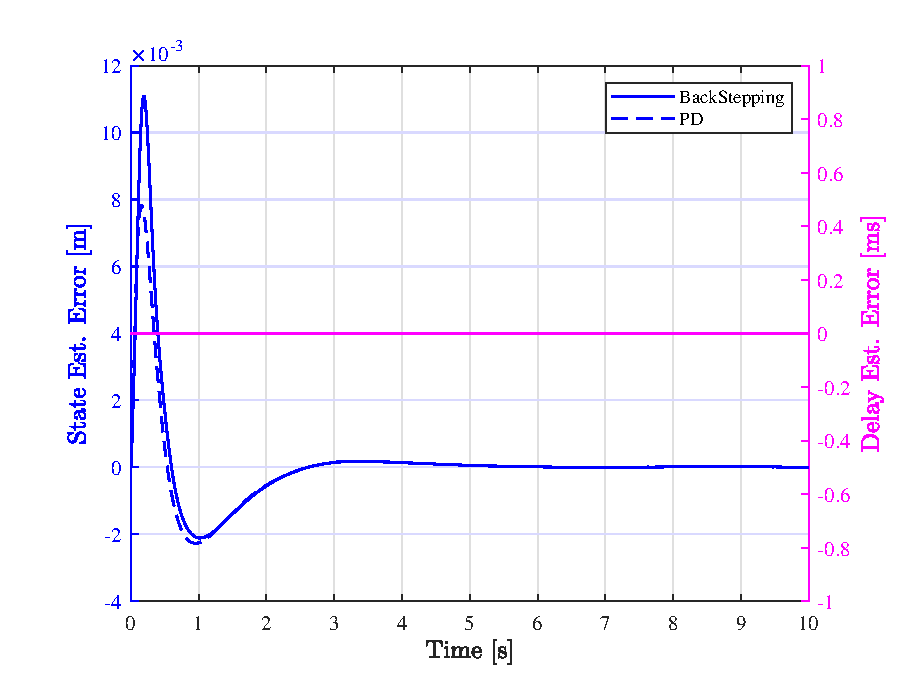
\includegraphics{Figures/RMSEPerfect.eps}}
	\caption{State estimation error with perfect delay estimator}
	\label{fig:Error(PerfectEstLow)}
\end{figure}

Fig.~\ref{fig:U(PerfectEstLow)} shows the control signals calculated on the  Ground Control Station according to the estimated quadrotor states. The control signal for both controllers are similar, and as it is shown in Fig.~\ref{fig:Error(PerfectEstLow)}, the control framework that works based on the PD controller estimates the states similar to the state estimator that works based on the backstepping.

\begin{figure}[H]
	\centerline{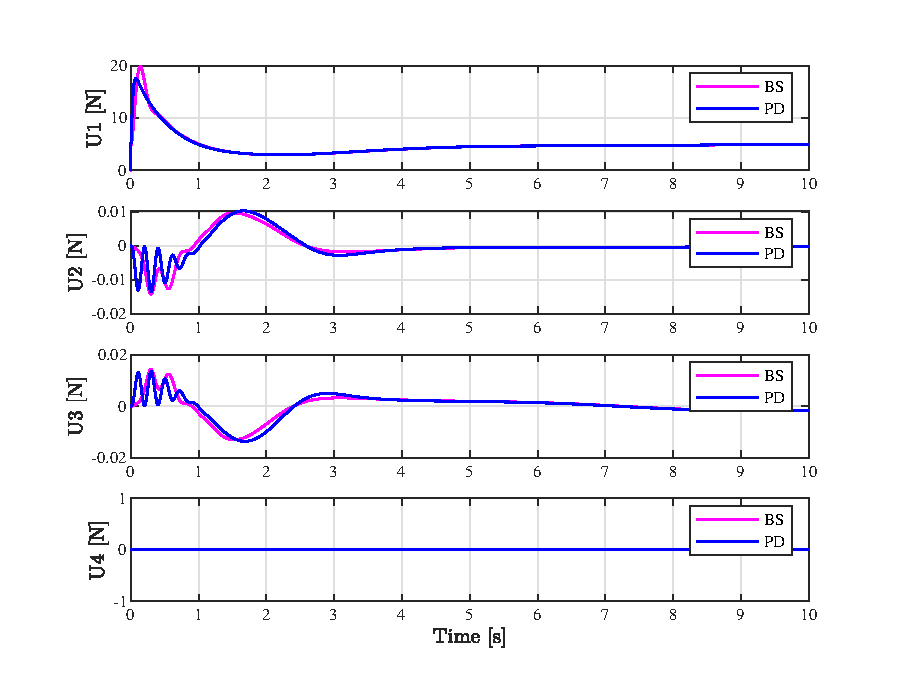
\includegraphics{Figures/UPerfect.eps}}
	\caption{Control signals with perfect delay estimator}
	\label{fig:U(PerfectEstLow)}
\end{figure}

\paragraph{Delay estimation based on the Markov model} In this case, delays were changed based on the predefined transition matrix. According to Fig.~\ref{fig:Error(NormalLow)}, the estimation error for the PD and backstepping controllers did not change significantly due to small delay values. The true and estimated transition probability matrices are shown in Table \ref{Table3.3}.

\begin{table}[H]
	\begin{center}
	\caption{True and estimated transition probabilities}
		\begin{tabular}{|clllll|}
		\hline
		\multicolumn{1}{|l}{}                     &                               & \multicolumn{1}{c}{6 $ms$} & \multicolumn{1}{c}{7 $ms$} & \multicolumn{1}{c}{9 $ms$} & \multicolumn{1}{c|}{10 $ms$} \\ \hline
		\multicolumn{1}{|c|}{\multirow{2}{*}{6 $ms$}}  & \multicolumn{1}{l|}{True}     & 0.7736                & 0.0250                & 0.1643                & 0.0372                  \\
		\multicolumn{1}{|c|}{}                    & \multicolumn{1}{l|}{Estimate} & 0.7631                & 0.0259                & 0.1705                & 0.0405                  \\ \hline
		\multicolumn{1}{|c|}{\multirow{2}{*}{7 $ms$}}  & \multicolumn{1}{l|}{True}     & 0.0224                & 0.1972                & 0.0723                & 0.7080                  \\
		\multicolumn{1}{|c|}{}                    & \multicolumn{1}{l|}{Estimate} & 0.0349                & 0.2170                & 0.0574                & 0.6908                  \\ \hline
		\multicolumn{1}{|c|}{\multirow{2}{*}{9 $ms$}}  & \multicolumn{1}{l|}{True}     & 0.0360                & 0.1797                & 0.0310                & 0.7533                  \\
		\multicolumn{1}{|c|}{}                    & \multicolumn{1}{l|}{Estimate} & 0.0333                & 0.1849                & 0.0258                & 0.7559                  \\ \hline
		\multicolumn{1}{|c|}{\multirow{2}{*}{10 $ms$}} & \multicolumn{1}{l|}{True}     & 0.2097                & 0.0075                & 0.0305                & 0.7523                  \\
		\multicolumn{1}{|c|}{}                    & \multicolumn{1}{l|}{Estimate} & 0.2174                & 0.0072                & 0.0357                & 0.7397                  \\ \hline
		\end{tabular}
		\label{Table3.3}
	\end{center}
\end{table}


\begin{figure}[H]
	\centering
	\centerline{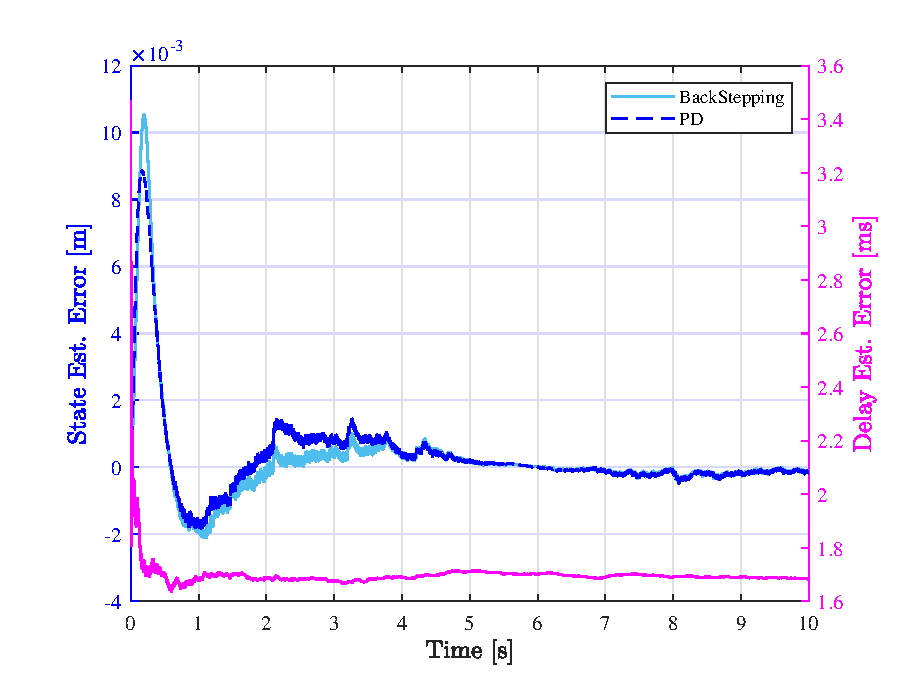
\includegraphics{Figures/RMSENormalLow.eps}}
	\caption{State and delay estimation error for $D=\left\lbrace 6, 7, 9, 10\right\rbrace$ $ms$}
	\label{fig:Error(NormalLow)}
\end{figure}

As illustrated in Fig.~\ref{fig:U(NormalLow)}, even very small unknown delays affect controller performance. Because of the time delay in the system, tiny oscillations happen in the quadrotor's orientation. For example, since the bandwidth of the PD controller is relatively high (large gains in the control signal), small feedback errors are multiplied by the large gains and generate oscillating control signals.

\begin{figure}[H]
	\centerline{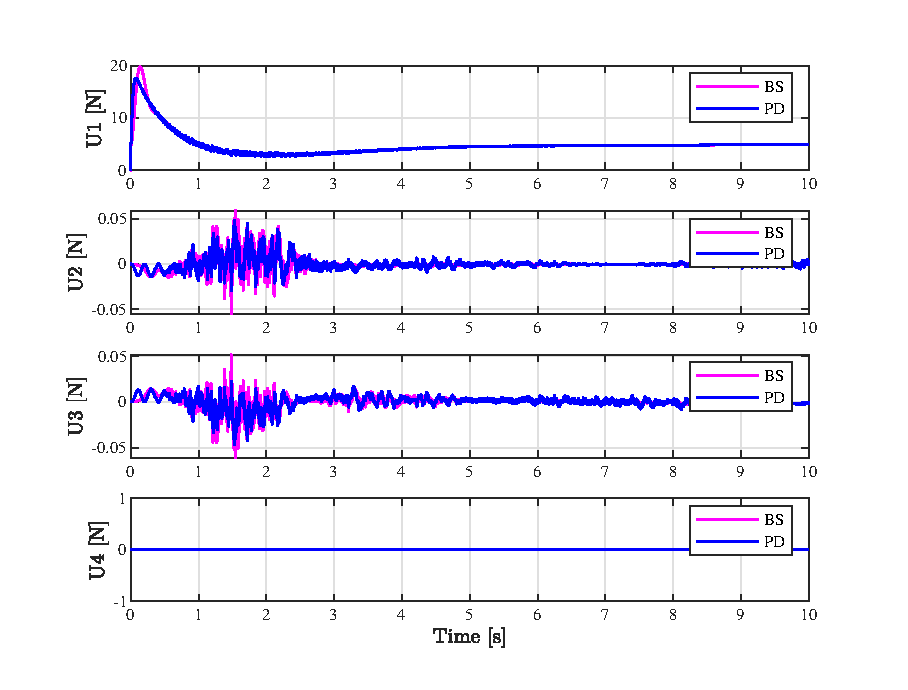
\includegraphics{Figures/UNormalLow.eps}}
	\caption{Control signals for $D=\left\lbrace 6, 7, 9, 10\right\rbrace$ $ms$}
	\label{fig:U(NormalLow)}
\end{figure}

In order to study the effect of the large changes in delay on the system, the time delays were changed to $D=\left\lbrace 1, 3, 13, 15\right\rbrace$ $ms$. The simulation was done with the true transition probabilities presented in Table \ref{Table3.3}. Fig.~\ref{fig:Error(NormalHigh)} shows how a slight change in the delay variation increases the estimation error. It also shows that we cannot use the mean value for the delay because large variations in delay negatively affect the response. It takes longer for the state estimator to estimate the current position.

\begin{figure}[H]
	\centering
	\centerline{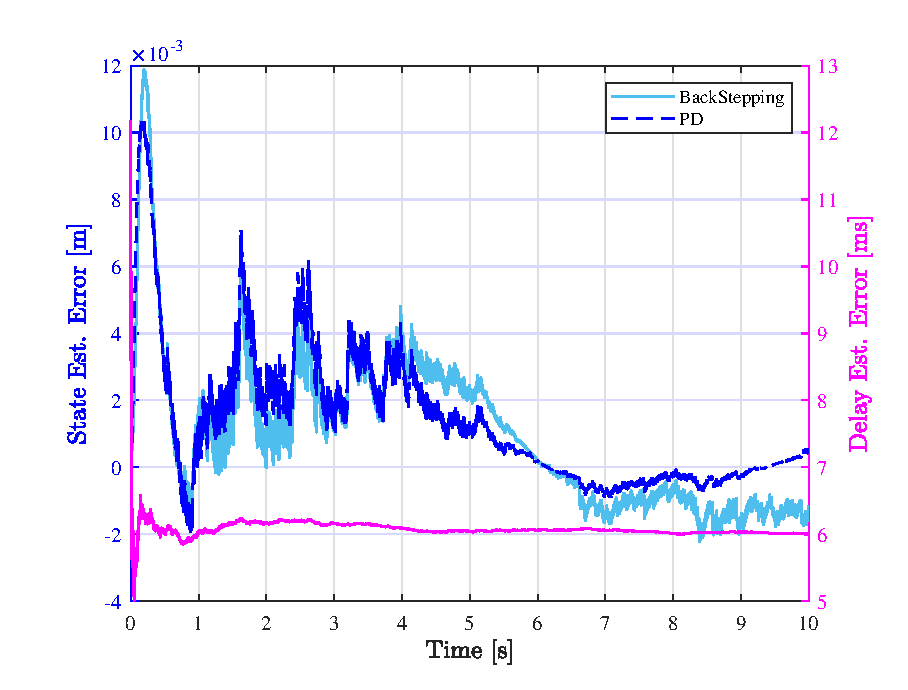
\includegraphics{Figures/RMSENormalHigh.eps}}
	\caption{State and delay estimation error for $D=\left\lbrace 1, 3, 13, 15\right\rbrace$ $ms$}
	\label{fig:Error(NormalHigh)}
\end{figure}

According to Fig.~\ref{fig:U(NormalHigh)}, large variations in state estimation error affect the backstepping controller so that it generates control signals with higher frequency and amplitude than the PD controller. It should be noted that although one way to solve this problem is to reduce the backstepping controller's coefficients, lower values for coefficients increase the response time and path RMSE.

\begin{figure}[H]
	\centerline{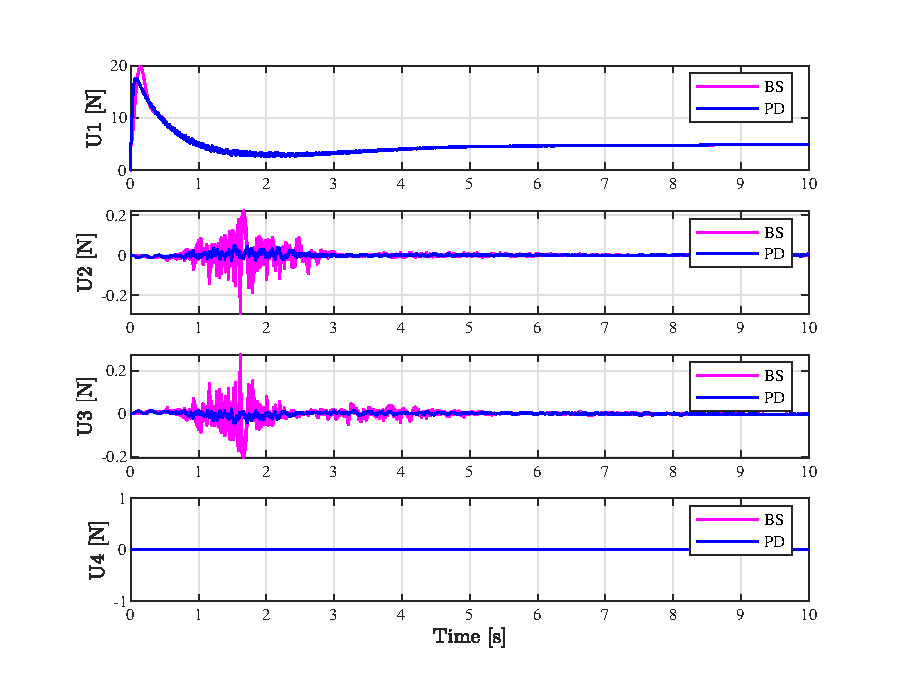
\includegraphics{Figures/UNormalHigh.eps}}
	\caption{Control signals for $D=\left\lbrace 1, 3, 13, 15\right\rbrace$ $ms$}
	\label{fig:U(NormalHigh)}
\end{figure}


\paragraph{Change in delay values and distributions} While the cellular networks provide higher communication bandwidth with lower time delays, the variation in network load in crowded areas like urban environments changes the network properties. During the simulation, the time delays ($D$) and their distributions $p$ were changed to simulate the changes in network states. The simulation was done with delays between $1-10$ $ms$, and the time delay values and their transition probabilities were changed six times.

\begin{figure}[H]
	\centerline{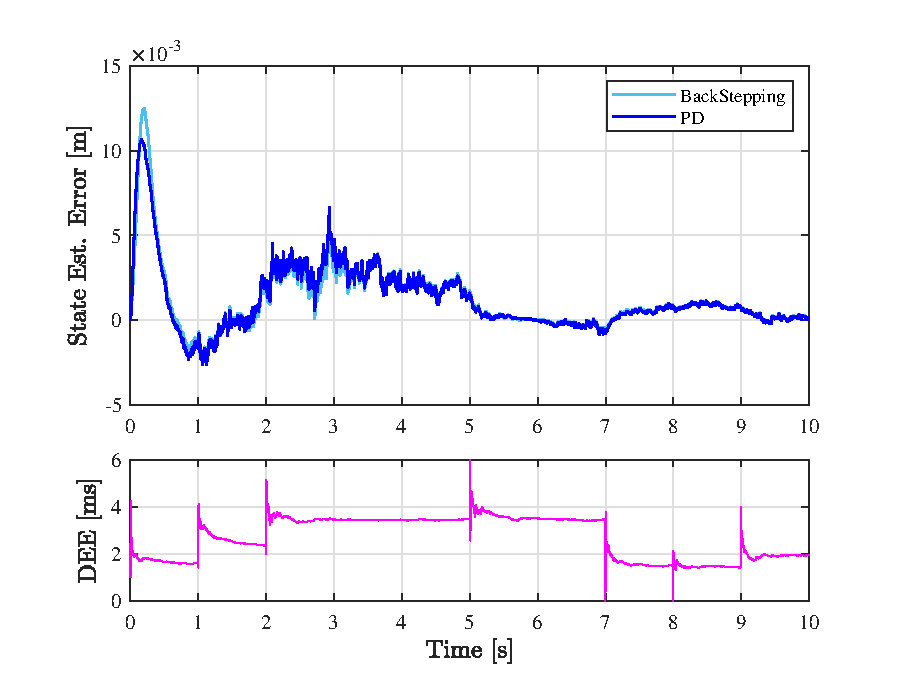
\includegraphics{Figures/RMSEDlyChng.eps}}
	\caption{State and delay estimation error when delays and their distribution changed (Large variations in delay estimation shows the points where the delay values and the transition probabilities are changed)}
	\label{fig:Error(DelayChng)}
\end{figure}

Fig.~\ref{fig:Error(DelayChng)} shows the delay estimation error during the simulation. According to the figure, change in delay values and distributions has affected the delay estimation. However, small delay changes between 1 to 10 $ms$ did not decrease the state estimator's performance. It should be noted that after every change in delay, the DEE was reset, and error was calculated for new time delays.

\begin{figure}[H]
	\centerline{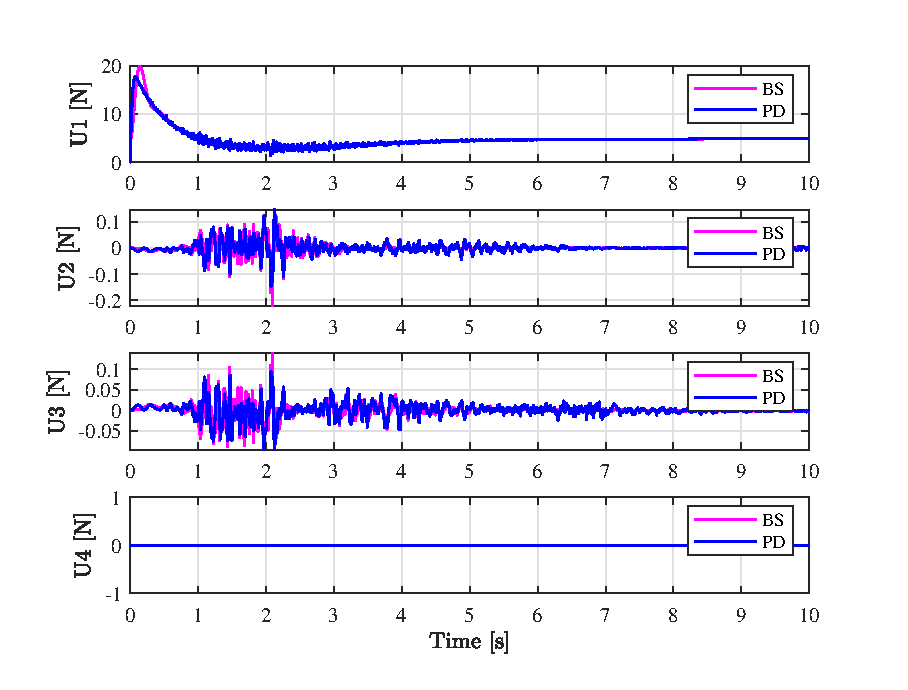
\includegraphics{Figures/UDelayChange.eps}}
	\caption{Control signals when delays and delay distributions changed}
	\label{fig:U(DelayChng)}
\end{figure}

As shown in Fig.~\ref{fig:U(DelayChng)}, errors in estimating time delay caused high-frequency oscillations in the control signal. Although the maximum delay value is not changed, changing delay values between 1 to 10 $ms$ negatively affected the control signal.

According to the results, PD and backstepping controllers have similar performance in quadrotor control. However, in the case of the large variation in time delay, the PD controller generates better control signals. The design process of the backstepping controller is more complicated than the PD controller.

In this chapter, the PD gains and backstepping coefficients were set so that the trajectory tracking performance was almost the same. RMSE of the path in $x$, $y$, and $z$ directions were 1.046, 1.138, and 0.131 $m$ for the PD controller, and 1.224, 1.329, and 0.19 $m$ for the backstepping controller. In this case, the forward delay is the major reason for high RMSE and makes quadrotor follow the path with delay. 

In the linear PD controller, the gains can be tuned using inner and outer loop bandwidths. Also, using the theoretical stability analysis based on the linearized model, one can find an equation between time delay and controller's bandwidth. This issue helps the control framework adjust the bandwidth based on the observed time delay. 

The bandwidth adaptation in the backstepping controller is a complex task since 12 parameters should be tuned. On the other hand, developing an equation between coefficients and time delay is much more complex than the linear PD controller.

Cellular networks are state-of-the-art communication tools for precise swarm control of drones. The presented control framework can control multiple drones from the GCS while the state estimator provides precise information about each drone's current position and orientation (fully observable system) for real-time centralized multi-agent-based collision avoidance, cooperation, and path planning tasks.

\section{Experimental setup}


\include{4_ATD_with_SNN}
\include{5_FL_with_SNN}
\include{6_Future_Work}


\bibliography{Ref}
\bibliographystyle{ieeetr}

\end{document}
